% !TeX program = pdflatex
% !TeX encoding = UTF-8
% !TeX spellcheck = pt_BR

\documentclass[12pt, a4paper, openright, oneside, brazil]{abntex2}

% Inclui o preâmbulo com todos os pacotes
% ----------------------------------------------------------------------------------------------------------------------
% Pacotes essenciais para a escrita do trabalho acadêmico;
% ----------------------------------------------------------------------------------------------------------------------
\usepackage[utf8]{inputenc}
\usepackage[T1]{fontenc}
\usepackage[brazil]{babel}
\usepackage{lmodern}
\usepackage{microtype}
\usepackage{graphicx}
\usepackage{color}
\usepackage{xcolor}
\usepackage{amsmath,amsfonts,amssymb}
\usepackage{indentfirst}
\usepackage{times}
\usepackage{url}
\usepackage{hyperref}
\usepackage{float}
\usepackage{listings}
\usepackage{caption}
\usepackage{subcaption}
\usepackage{longtable}
\usepackage{tabularx}
\usepackage{booktabs}
\usepackage{array}
\usepackage{fancyhdr}
\usepackage{abntex2cite} % Citações padrão ABNT
\usepackage{geometry}
\usepackage{url}
% Inclui as configurações
% ----------------------------------------------------------------------------------------------------------------------
% Definindo minhas cores bases;
% ----------------------------------------------------------------------------------------------------------------------
\definecolor{branco}{HTML}{FFFFFF}
\definecolor{roxoescuro}{HTML}{1E1647}
\definecolor{roxoclaro}{HTML}{614AD3}
\definecolor{amarelo}{HTML}{FFFF00}
% ----------------------------------------------------------------------------------------------------------------------
% Configurações para ambiente de código;
% ----------------------------------------------------------------------------------------------------------------------
\lstdefinestyle{custom}{
    backgroundcolor=\color{branco},
    basicstyle=\footnotesize\ttfamily,
    breaklines=true,
    frame=single,
    rulecolor=\color{roxoescuro},
    upquote=true
}
% ----------------------------------------------------------------------------------------------------------------------
% Configurações de Links;
% ----------------------------------------------------------------------------------------------------------------------
\hypersetup{
    colorlinks=true,
    linkcolor=roxoescuro,
    filecolor=amarelo,
    urlcolor=roxoclaro,
    pdftitle={Guia Prático para a Capacitação em GitHub},
    pdfpagemode=FullScreen,
    pdfauthor={Ronivaldo Domingues de Andrade},
    pdfsubject={Capacitação em GitHub},
    pdfkeywords={GitHub, Controle de Versão, Colaboração, Repositórios, Branches, Commits, Pull Requests, CI/CD}
}
% ----------------------------------------------------------------------------------------------------------------------
% Configurações do lstset do listings
% ----------------------------------------------------------------------------------------------------------------------
\lstset{
    backgroundcolor=\color{gray!10},
    basicstyle=\ttfamily\footnotesize,
    breaklines=true,
    frame=single,
    numbers=left,
    numberstyle=\tiny\color{gray},
    captionpos=b
}

% Informações para CAPA e FOLHA DE ROSTO
\title{Capacitação em GitHub}
\author{Ronivaldo Domingues de Andrade}
\local{Rio de Janeiro - RJ}
\data{2025}
\tipotrabalho{Guia Prático para Capacitação}
\preambulo{Guia Prático para Capacitação em GitHub}

\begin{document}
\selectlanguage{brazil}

% Elementos pré-textuais
\imprimircapa
\imprimirfolhaderosto

\newpage
\listoffigures

\newpage
\listoftables

% Lista de siglas
\begin{siglas}
  \item[Winget] Windows Package Manager
  \item[GitHub] Plataforma de Controle de Versão Distribuído
  \item[git] Sistema de Controle de Versão Distribuído
  \item[gh] GitHub CLI (Command Line Interface)
  \item[git-lfs] Sistema de Controle de Versão Distribuído para Arquivos Grandes
  \item[Merge] Fusão de Branches no GitHub
  \item[Branch] Rama (branch) em um repositório GitHub
  \item[Commit] Confirmação de Modificações em um Branch
  \item[GitHub Pages] Serviço de Hospedagem de Páginas Estáticas
  \item[GitHub Actions] Plataforma de Automação de Fluxos de Trabalho
  \item[Pull Request (PR)] Solicitação de Mesclagem de Código
  \item[Markdown] Linguagem de Marcação Leve
  \item[README] Arquivo de Documentação do Projeto
  \item[.gitignore] Arquivo de Configuração para Ignorar Arquivos no Git
  \item[LICENSE] Arquivo de Licença do Projeto
  \item[MIT] Licença MIT -> Massachusetts Institute of Technology License
  \item[YML] YAML Ain't Markup Language -> YAML Não é uma Linguagem de Marcação de Texto, mas sim uma sintaxe para arquivos YAML
  \item[GPG] GNU Privacy Guard -> Guarda de Privacidade GNU, ferramenta de criptografia de dados e comunicação segura.
\end{siglas}

\tableofcontents

% Capítulos do trabalho
% ----------------------------------------------------------------------------------------------------------------------
% Início dos capítulos do trabalho;
% ----------------------------------------------------------------------------------------------------------------------
\chapter{Introdução}

O GitHub consolidou-se como uma das principais plataformas de desenvolvimento colaborativo, sendo amplamente adotado por equipes e desenvolvedores individuais para o controle de versão, a gestão de projetos e a integração contínua. No entanto, o uso eficiente de suas ferramentas exige não apenas familiaridade com conceitos básicos, mas também o domínio de boas práticas e fluxos de trabalho modernos.

Esta capacitação foi elaborada com o objetivo de oferecer um guia prático e acessível para o uso do GitHub e de suas tecnologias associadas, como Git, GitHub CLI, Git LFS, GitHub Pages e GitHub Actions. O material abrange desde a configuração inicial do ambiente até a execução de operações avançadas, como a assinatura de commits com GPG e a automação de fluxos de trabalho.

Além disso, são apresentados exercícios práticos que simulam situações reais de desenvolvimento, permitindo que os participantes vivenciem todo o ciclo de colaboração em projetos versionados. Com isso, espera-se que, ao final do curso, os participantes estejam aptos a contribuir de forma segura, organizada e profissional em repositórios locais e remotos, seja em projetos pessoais ou corporativos.    % Introdução
\chapter{GitHub}
\par
\section{O que é?}
O GitHub é uma plataforma de hospedagem de código-fonte que utiliza o sistema de controle de versão Git. Ele permite que desenvolvedores colaborem em projetos, compartilhem código e gerenciem alterações de forma eficiente. Com o GitHub, é possível criar repositórios, realizar pull requests, revisar código e acompanhar o histórico de alterações.
\par
Além disso, o GitHub oferece recursos adicionais, como GitHub Pages para hospedagem de sites estáticos, GitHub Actions para automação de fluxos de trabalho e integração com diversas ferramentas de desenvolvimento.
\par
O GitHub é amplamente utilizado na indústria de software, sendo uma ferramenta essencial para desenvolvedores, equipes de desenvolvimento e organizações que buscam melhorar a colaboração e a gestão de projetos de software.
\par
\section{Criando seu perfil no GitHub}
Para criar uma conta no GitHub, siga os passos abaixo:
\begin{enumerate}
  \item Acesse o site do GitHub: \url{https://github.com/}
  \item Clique em "Sign up" no canto superior direito.
  \item Preencha os campos solicitados, como endereço de e-mail, nome de usuário e senha - Figura \ref{fig:signup_page}, p.\pageref{fig:signup_page}.
  \begin{figure}[H]
    \centering
    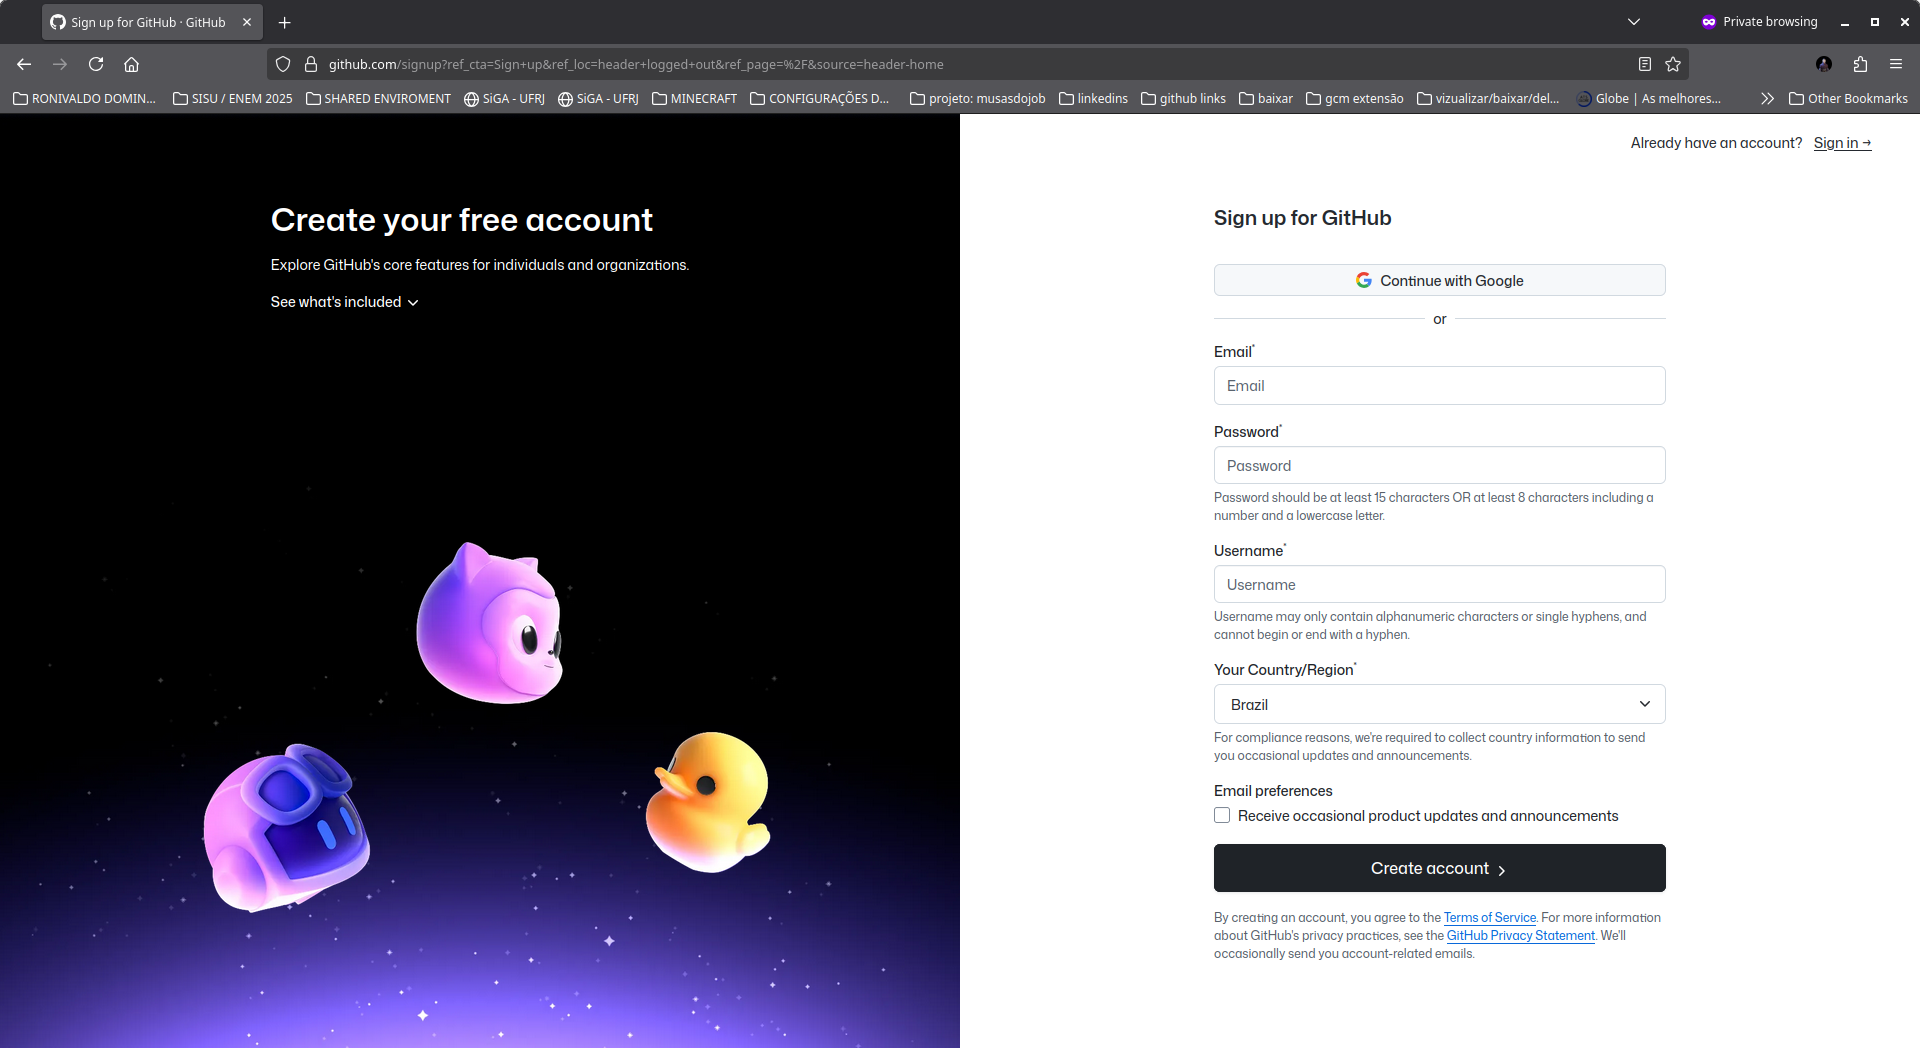
\includegraphics[width=0.8\textwidth]{./assets/images/01_signup_page.png}
    \caption{Página para a criação de conta no GitHub}
    \label{fig:signup_page}
  \end{figure}
  \item Siga as instruções na tela para concluir o processo de criação da conta.
  \item Ao final você verá a tela inicial do GitHub - Figura \ref{fig:signed_page}, p.\pageref{fig:signed_page}.
  \begin{figure}[H]
    \centering
    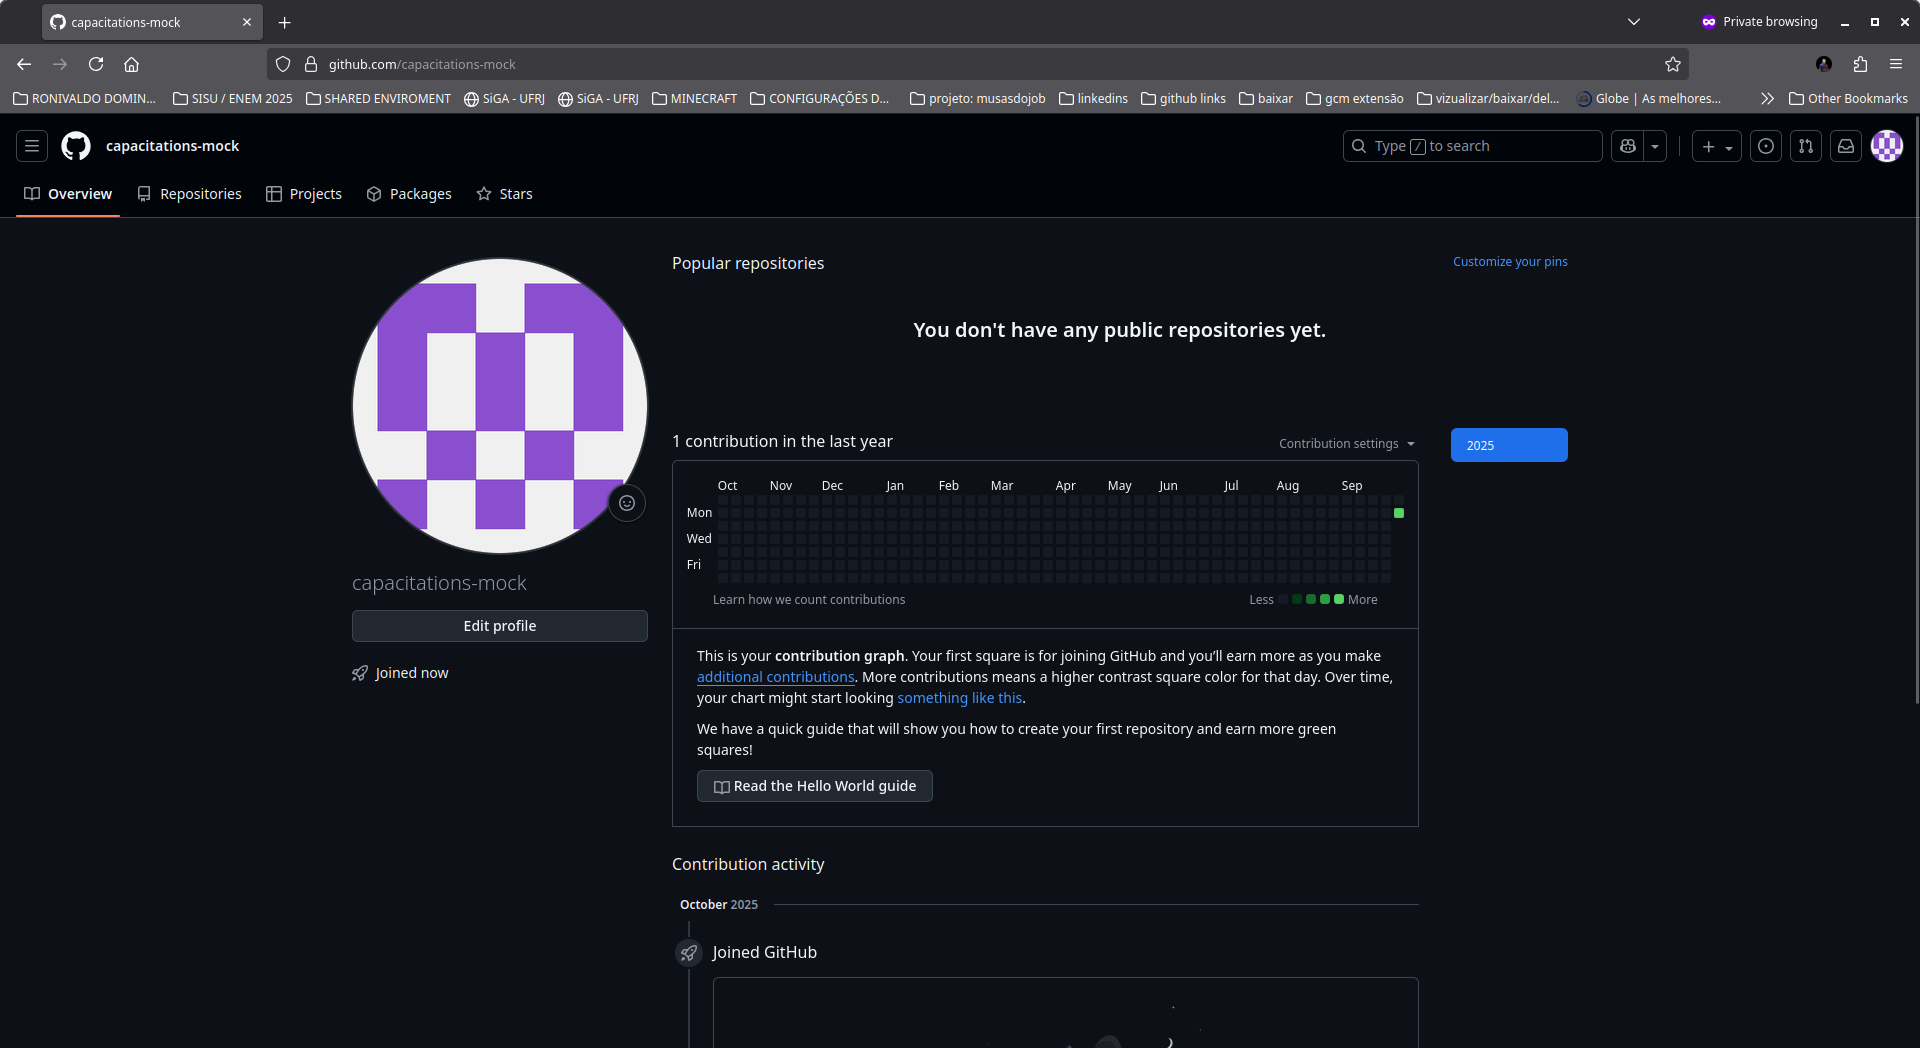
\includegraphics[width=0.8\textwidth]{./assets/images/02_signed_page.png}
    \caption{Primeira visão do GitHub depois de criar a conta}
    \label{fig:signed_page}
  \end{figure}
\end{enumerate}
\par
Após criar a conta, você poderá acessar o GitHub e começar a explorar seus recursos.
\par
\subsection{E-mail acadêmico e GitHub Student Developer Pack}
Para usar o GitHub Student Developer Pack e tornar sua conta uma GitHub Pro, você deve associar um e-mail acadêmico à sua conta. Isso pode ser feito nas configurações da conta, na seção "Emails". Adicionar um e-mail acadêmico pode ajudar a validar sua identidade como estudante ou profissional da área de tecnologia.
\par
Com isso o GitHub Student Developer Pack fornece acesso gratuito a diversas ferramentas e serviços para estudantes. Para se inscrever, você precisará verificar seu status de estudante com um e-mail acadêmico válido.
\par
\subsubsection{Por que usar o GitHub Student Developer Pack?}
O GitHub Student Developer Pack oferece uma série de benefícios, incluindo acesso gratuito a ferramentas de desenvolvimento, serviços de hospedagem e outros recursos que podem ser extremamente úteis para estudantes que estão aprendendo a programar e desenvolver software.
\par
\subsubsection{GitHub Free vs GitHub Student Developer Pack (GSDP)}
A conta gratuita do GitHub oferece recursos básicos, como repositórios públicos e privados, colaboração em projetos e integração com outras ferramentas. Já a conta GitHub Student Developer Pro oferece benefícios adicionais, como acesso a ferramentas premium, maior capacidade de armazenamento e recursos avançados de colaboração.
\par
\newpage
\subsubsection{GitHub Free vs GSDP}
\begin{table}[h!]
    \centering
    \begin{tabularx}{\textwidth}{|p{3cm}|p{3cm}|p{3cm}|X|}
        \hline
        \textbf{Recurso / Limite} & \textbf{GitHub Free (Conta Pessoal)} & \textbf{GitHub Student Developer Pack (GSDP)} & \textbf{Diferencial Estratégico} \\
        \hline
        Acesso a Repositórios Privados & Ilimitado (Recursos Limitados) & Ilimitado (Recursos Pro/Avançados) & Governança de Código \\
        \hline
        Minutos do GitHub Actions (Mensal) & 2,000 minutos & 3,000 minutos & Maior Resiliência de CI/CD (+50\%) \\
        \hline
        Armazenamento de Packages & 500 MB & 2 GB & Suporte a Artefatos e Contêineres (+400\%) \\
        \hline
        Horas de Core do Codespaces (Mensal) & 120 horas & 180 horas & Desenvolvimento em Nuvem Estendido \\
        \hline
        Armazenamento Codespaces (Mensal) & 15 GB & 20 GB & Maior Capacidade de Workspace \\
        \hline
        Revisores Obrigatórios (Private Repos) & Não Disponível & Disponível (Recurso Pro) & Enforçamento de Qualidade e Compliance \\
        \hline
        Suporte & Suporte Comunitário & Suporte Comunitário & Base de Suporte \\
        \hline
        Acesso ao GitHub Copilot & Não Incluído (Subscrição Paga) & Incluído (Geralmente Copilot Pro) & Produtividade e Aceleração por IA \\
        \hline
    \end{tabularx}
    \caption{GitHub Free (Pessoal) vs. GitHub Student Developer Pack (Pro)}
    \label{tab:core_comparison}
\end{table}
\par
\newpage
\section{Obtendo o GitHub Student Developer Pack}
\begin{enumerate}
  \item Vá até as configurações da sua conta no GitHub.
  \item Na seção "Emails", adicione seu e-mail acadêmico - Figura \ref{fig:adding_academic_email}, p.\pageref{fig:adding_academic_email}.
  \begin{figure}[H]
    \centering
    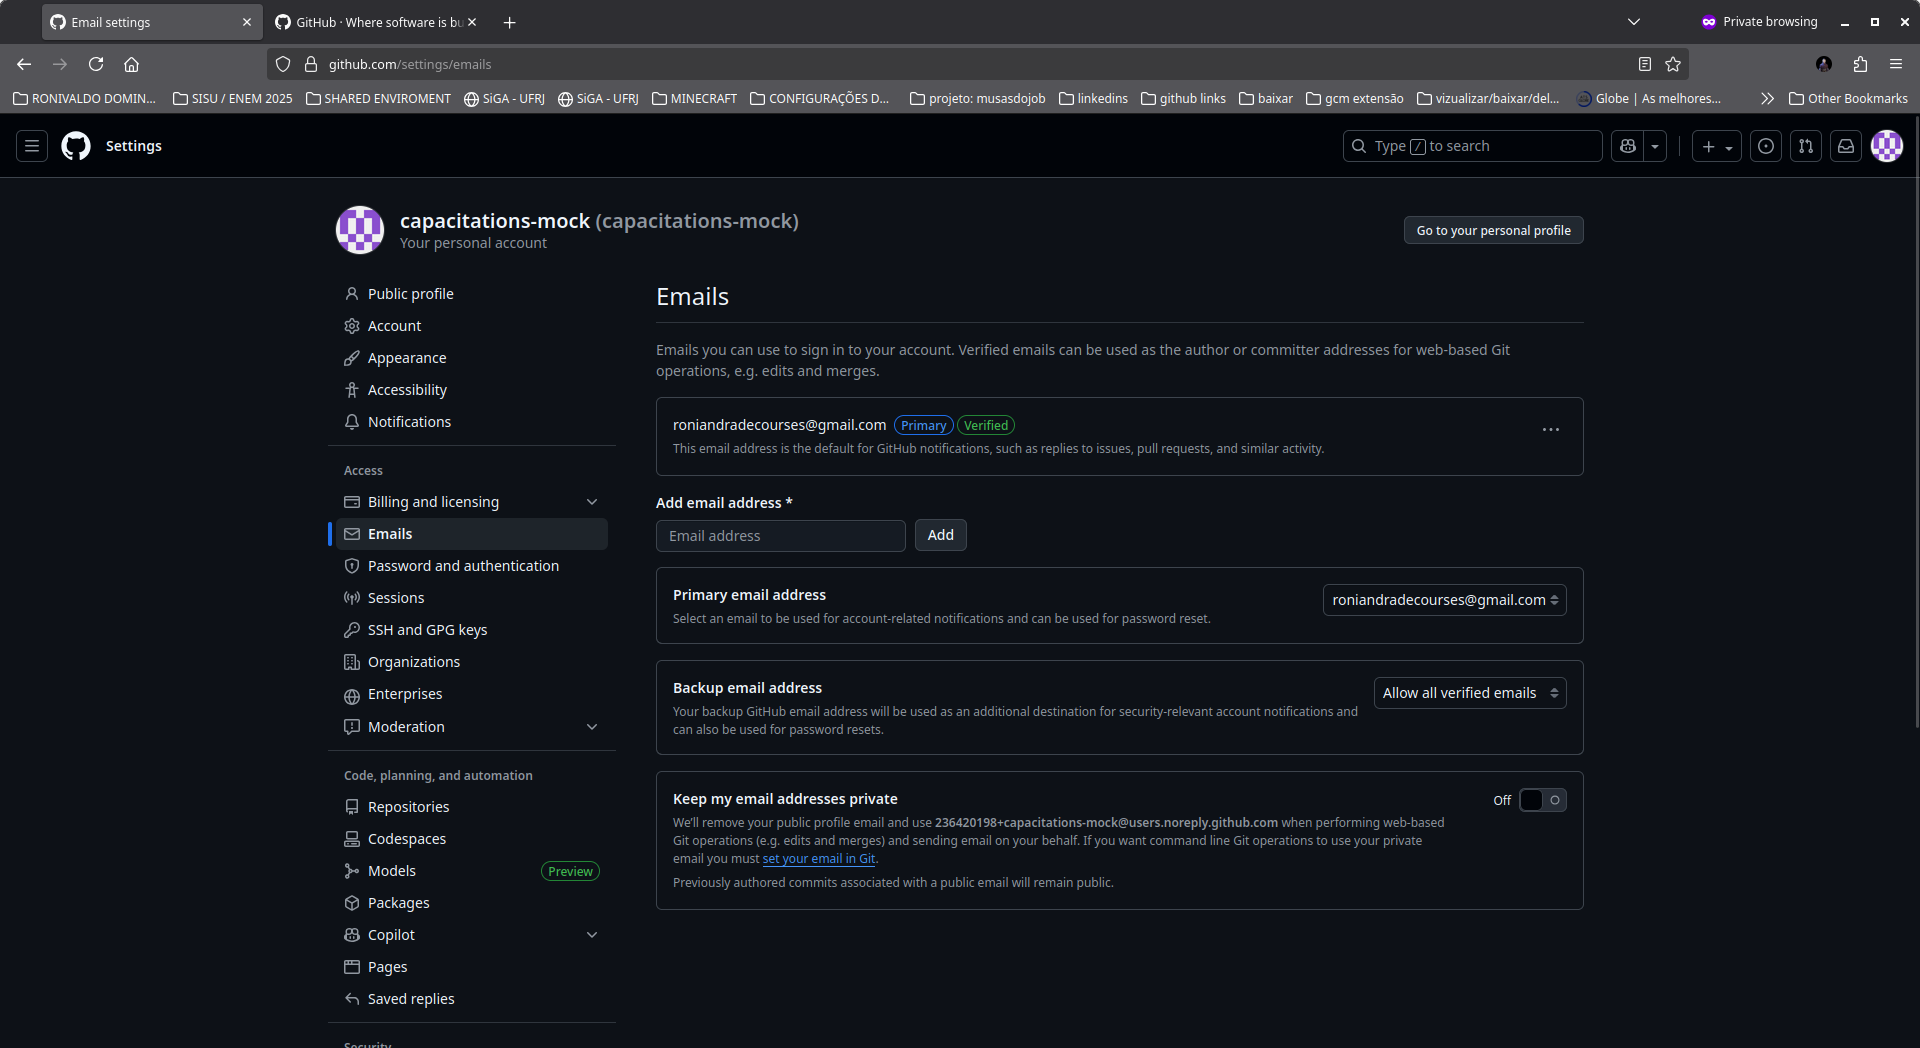
\includegraphics[width=0.9\textwidth]{./assets/images/03_adding_academic_email.png}
    \caption{Adicionar e verificar e-mail acadêmico no GitHub}
    \label{fig:adding_academic_email}
  \end{figure}
  \item Clique em "Add" \; para adicionar o e-mail.
  \item Verifique o e-mail clicando no link enviado para sua caixa de entrada.
  \item Após verificar o e-mail, você pode se inscrever no GitHub Student Developer Pack.
  \item Acesse o site do GitHub Student Developer Pack: \url{https://education.github.com/pack} - Figura \ref{fig:github_student}, p.\pageref{fig:github_student}.
  \begin{figure}[H]
    \centering
    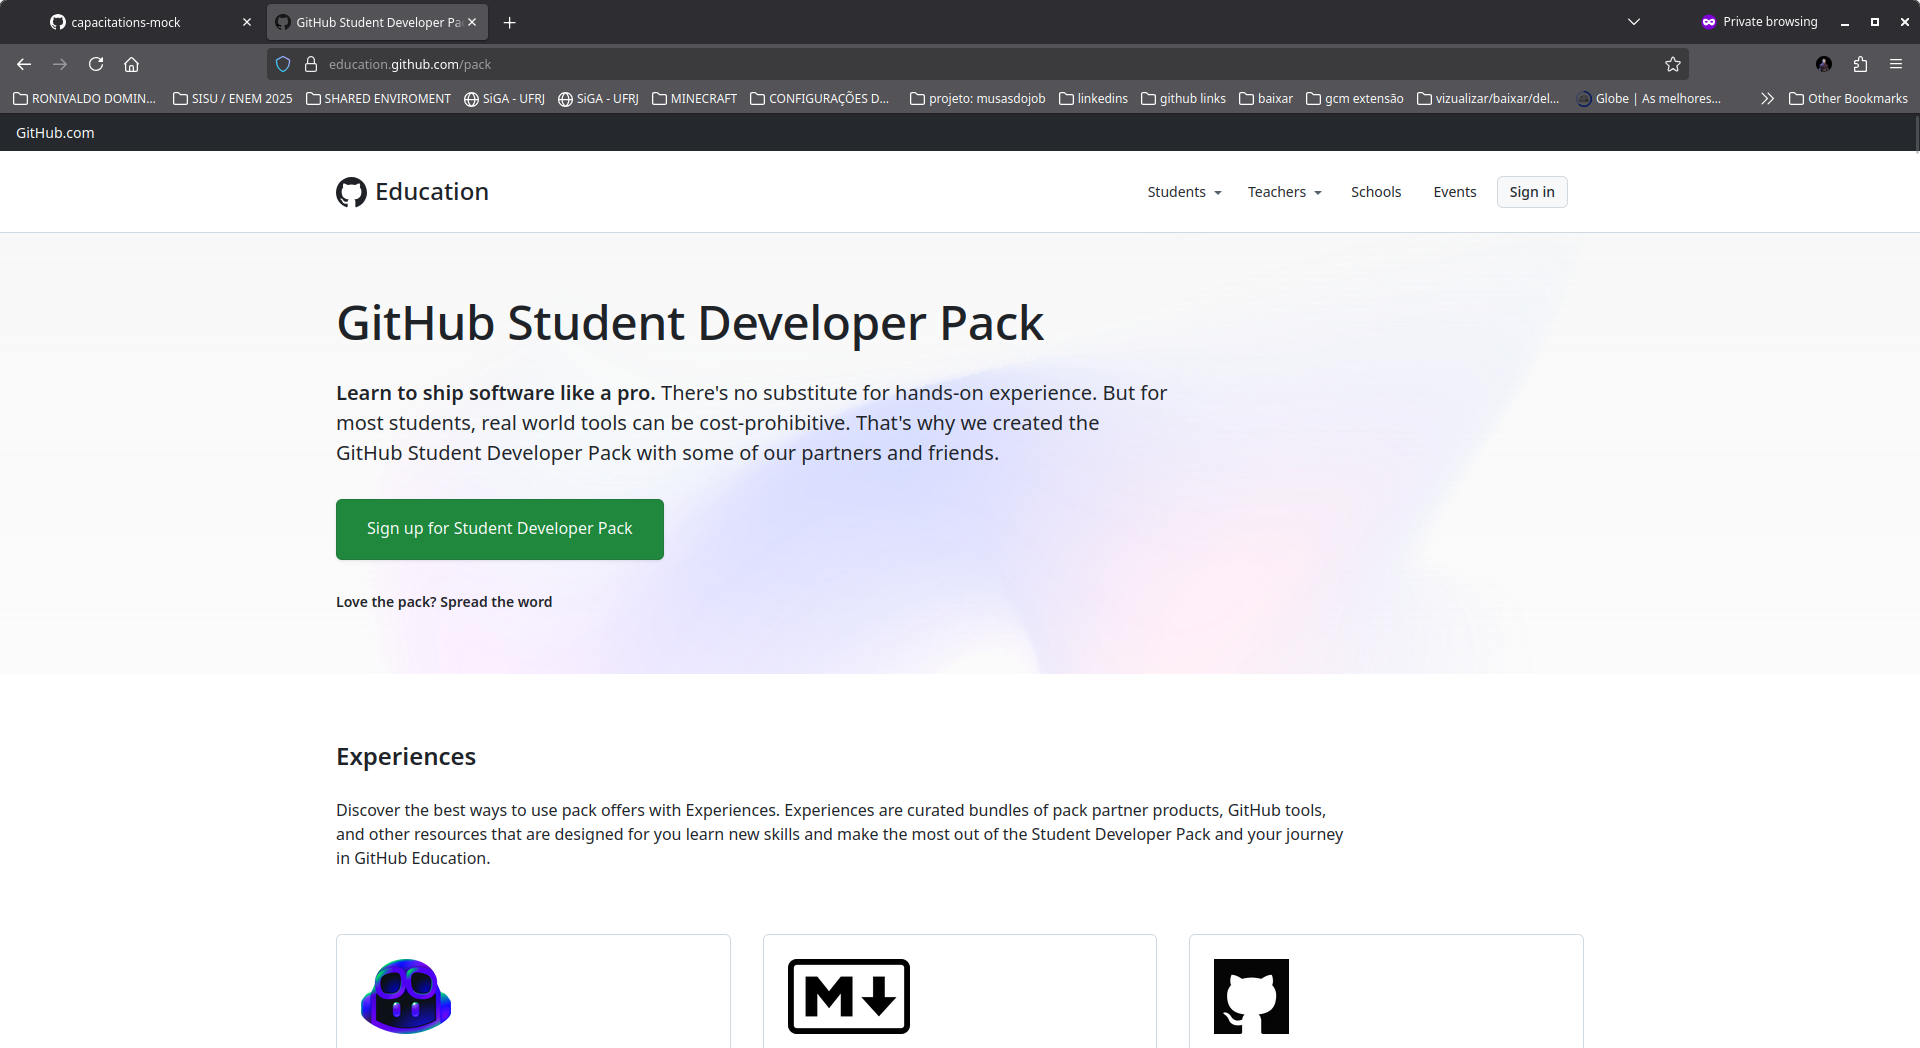
\includegraphics[width=0.9\textwidth]{./assets/images/04_gsdp_page.png}
    \caption{Página do GitHub Student Developer Pack}
    \label{fig:github_student}
  \end{figure}
  \item Clique em "Sign up for Student Developer Pack".
  \item Isso redirecionará para fazer login na sua conta do GitHub, caso não esteja logado - Figura \ref{fig:github_student_developer_pack}, p.\pageref{fig:github_student_developer_pack}.
  \begin{figure}[H]
    \centering
    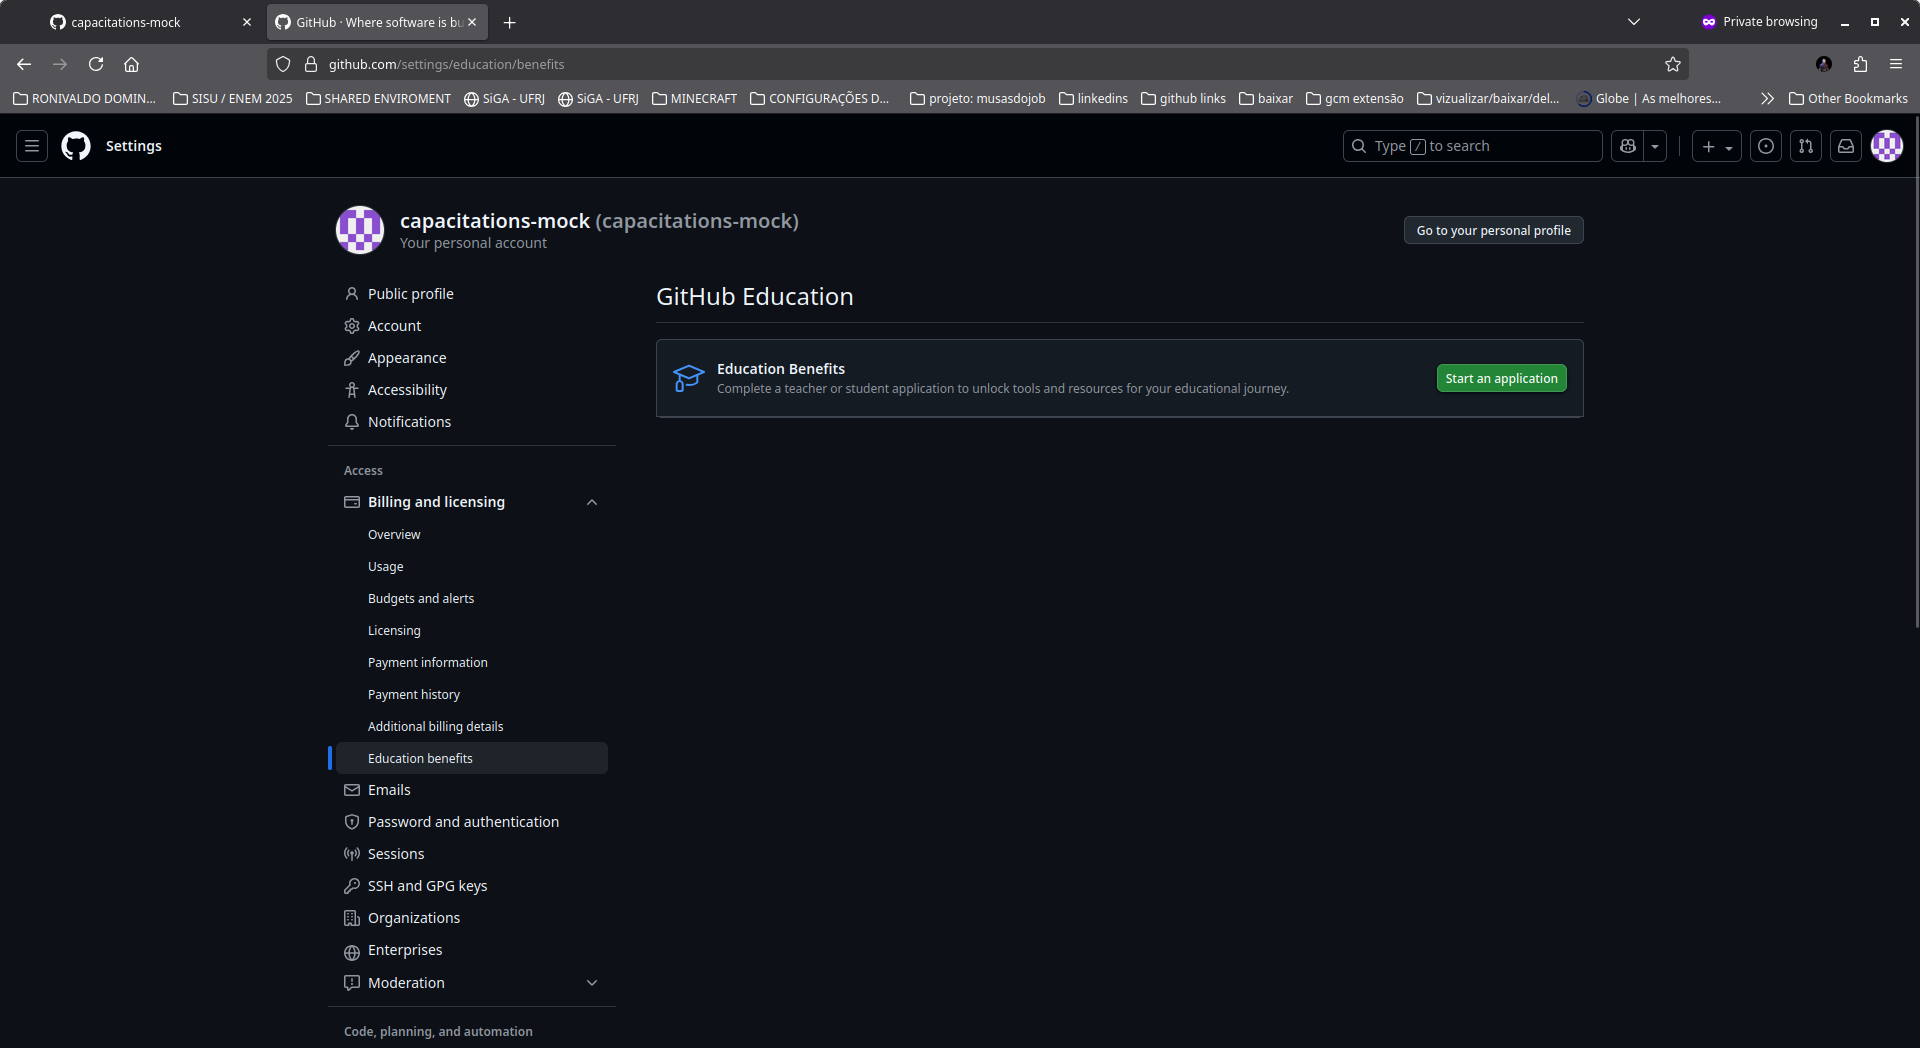
\includegraphics[width=0.9\textwidth]{./assets/images/05_application_page.png}
    \caption{Página do GitHub Student Developer Pack}
    \label{fig:github_student_developer_pack}
  \end{figure} 
  \item Preencha os campos solicitados, incluindo seu e-mail acadêmico - Figura \ref{fig:application_start}, p.\pageref{fig:application_start}.
  \begin{figure}[H]
    \centering
    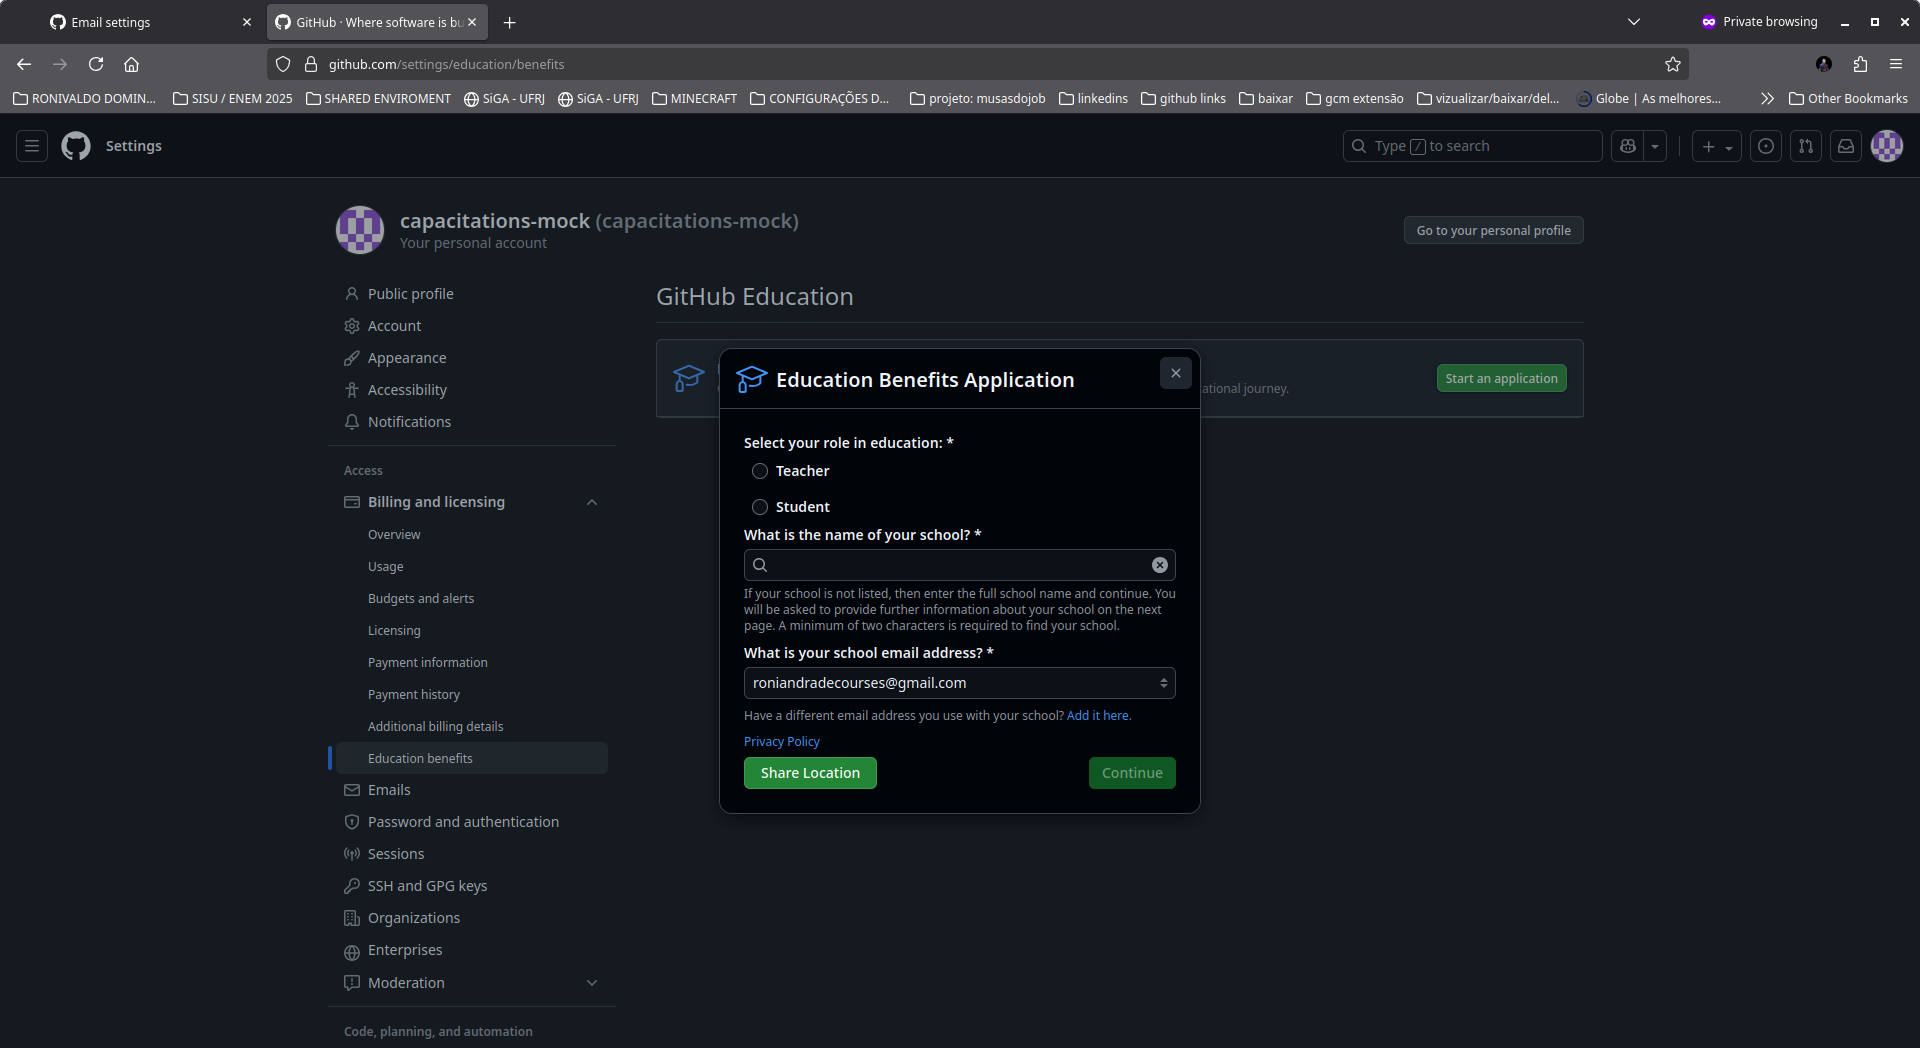
\includegraphics[width=0.9\textwidth]{./assets/images/06_start_application.png}
    \caption{Iniciando a aplicação no GitHub Student Developer Pack}
    \label{fig:application_start}
  \end{figure}
  \item Anexe um comprovante de matrícula ou uma carta da instituição de ensino, se solicitado. \textbf{(Importante: Use um documento oficial da instituição, por experiência própria, use a carteirinha de estudante que possui foto, para mim o processo foi mais rápido ao usar.)}
  \item Envie a solicitação e aguarde a aprovação, que pode levar alguns dias.
\end{enumerate}
\par    % GitHub
\chapter{Winget}
\par
\section{O que é?}
O Winget, ou Windows Package Manager, é uma ferramenta de linha de comando para Windows que permite instalar, atualizar e gerenciar aplicativos de forma simples e eficiente. Ele foi desenvolvido pela Microsoft e é uma solução nativa para gerenciamento de pacotes no Windows.

Para maiores informações e entendimento veja a documentação em \cite{microsoft_winget}.
\par
\section{Porque usar nessa capacitação?}
Para que todos possam acompanhar de maneira eficaz essa capacitação, preciso que todos tenham as ferramentas git e GitHub CLI instaladas em suas máquinas. Para facilitar esse processo, utilizaremos o Winget, que é o gerenciador de pacotes nativo do Windows.
O Winget é um gerenciador de pacotes para Windows que facilita a instalação, atualização e remoção de aplicativos. Com ele, é possível automatizar a configuração do ambiente de desenvolvimento, economizando tempo e esforço.
\par
\subsection{Instalação}
\par
\begin{citacao}
A ferramenta de linha de comando do WinGet só tem suporte no Windows 10 versão 1809 (build 17763) ou posterior. 
O WinGet não estará disponível até que você tenha feito logon no Windows como usuário pela primeira vez, 
o que fará com que a Microsoft Store registre o Gerenciador de Pacotes do Windows como parte de um processo assíncrono. 
Se você tiver feito logon recentemente como usuário pela primeira vez e o WinGet ainda não estiver disponível, 
abra o PowerShell e insira o seguinte comando para solicitar o registro dele: 

\texttt{Add-AppxPackage -RegisterByFamilyName -MainPackage Microsoft.DesktopAppInstaller\_8wekyb3d8bbwe.}
\citeonline{microsoft_winget}.
\end{citacao}

\begin{enumerate}
  \item Verifique se o Winget já está instalado no seu sistema. Abra o Prompt de Comando ou PowerShell e digite
  \begin{verbatim}
    winget --version
  \end{verbatim}
  Se o comando retornar uma versão, o Winget já está instalado.
  \begin{figure}[H]
    \centering
    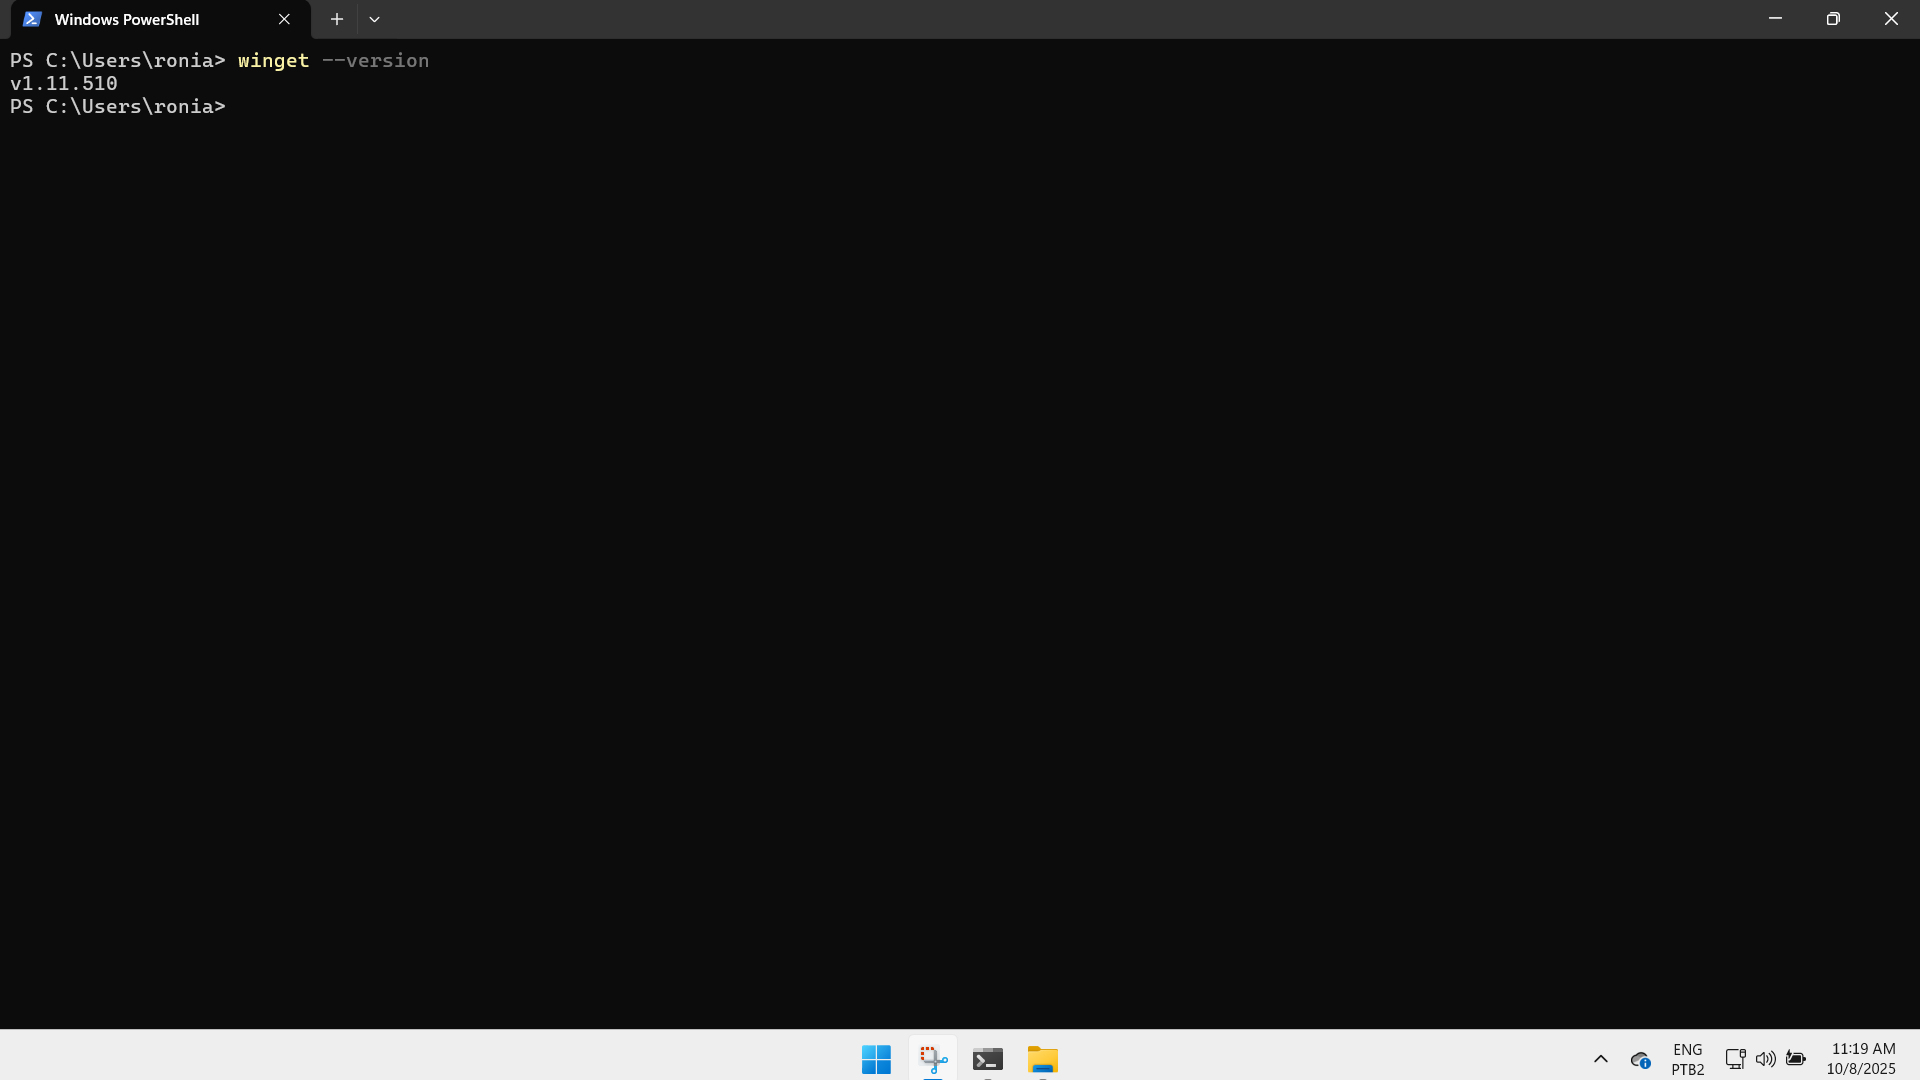
\includegraphics[width=0.9\textwidth]{./assets/images/07_winget_installed.png}
    \caption{Verificando se o Winget está instalado.}
    \label{fig:winget_installed}
  \end{figure}
  \item Caso o Winget não esteja instalado, você pode baixá-lo como parte do aplicativo "App Installer" da Microsoft Store. Acesse a Microsoft Store, procure por "App Installer" e clique em "Obter" para instalar. Caso enfrente alguma dificuldade, acesse a documentação em \cite{microsoft_winget}.
  \item Após a instalação, reinicie o Prompt de Comando ou PowerShell e verifique novamente a instalação com:
  \begin{verbatim}
    winget --version
  \end{verbatim}
  O comando deve retornar a versão do Winget instalada.
\end{enumerate}
\par
\subsubsection{Atualização}
Para garantir que você está utilizando a versão mais recente do Winget, execute o comando:
\begin{verbatim}
  winget upgrade --all
\end{verbatim}
Este comando atualizará todos os pacotes instalados, incluindo o próprio Winget, se houver uma atualização disponível.    % Winget
\chapter{Git e GitHub-CLI}
\par
\section{O que é o Git?}
O Git é um software open source, gratuito e multiplataforma voltado para o versionamento de código. Ele oferece um sistema de controle de versão distribuído, amplamente utilizado no desenvolvimento de software, que permite que múltiplos desenvolvedores trabalhem simultaneamente em um mesmo projeto. O Git rastreia as alterações realizadas nos arquivos, possibilitando reverter modificações, comparar versões e gerenciar ramificações (branches) de forma eficiente e segura.
\subsection{Instalação do Git}
\begin{enumerate}
  \item Abra o Prompt de Comando ou PowerShell.
  \item Digite o comando:
  \begin{verbatim}
    winget search git
  \end{verbatim}
  \item Na primeira vez que algum comando do Winget for executado, ele pedirá o aceite dos termos de uso. Ao aceitar, digitando \texttt{Y} ou \texttt{y}.
  \item Nesse comando \texttt{winget search git}, será buscado na base do winget todas as ocorrências em que o termo \texttt{git} aparece e será retornado uma tabela com os resultados associando o nome do programa, seu \textcolor{cyan}{id} para a instalação e algumas outras informações.
  \begin{figure}[H]
    \centering
    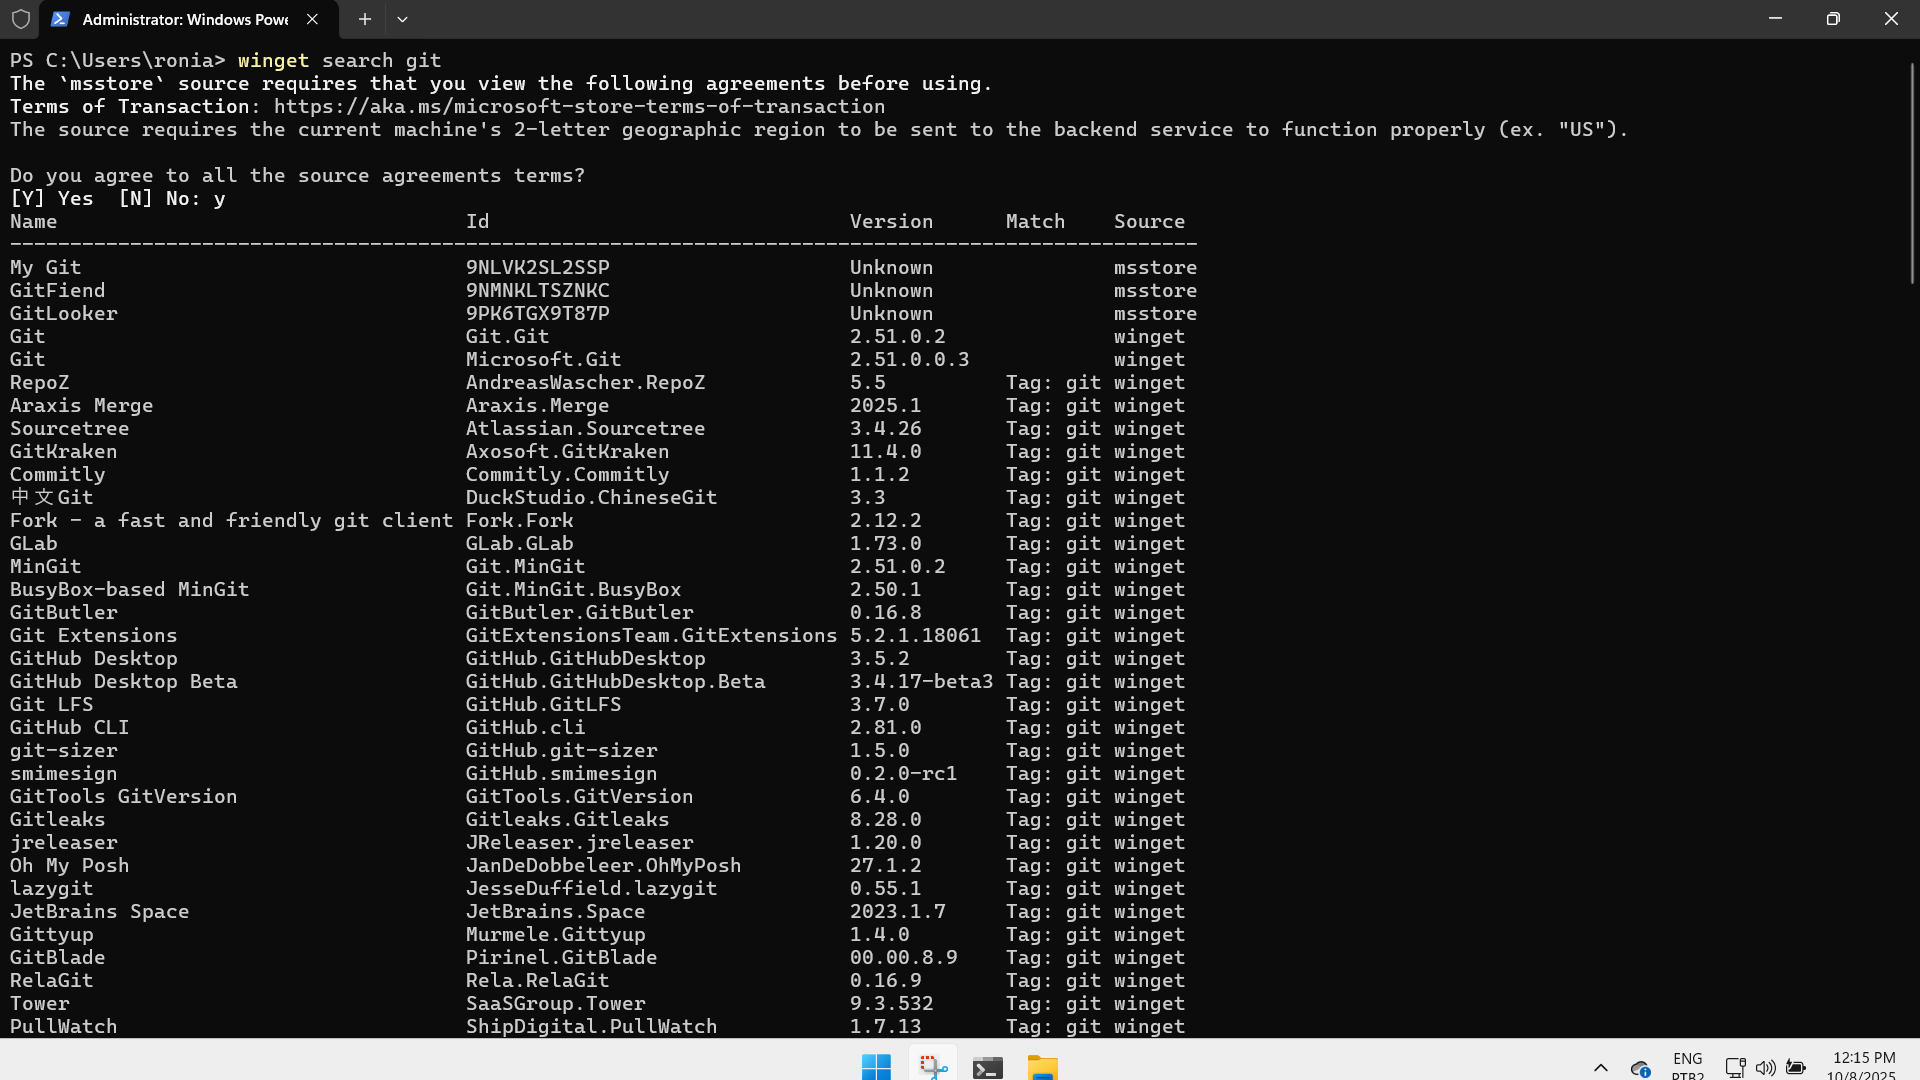
\includegraphics[width=0.9\textwidth]{./assets/images/08_winget_search.png}
    \caption{Buscando o Git no Winget.}
    \label{fig:winget_search}
  \end{figure} 
  \item Assim que localizar o software que deseja, copie ou memorize seu \textcolor{cyan}{id}, em nosso caso o \textcolor{cyan}{id} = \textcolor{cyan}{Git.Git}, e digite o comando:
  \begin{verbatim}
    winget install Git.Git
  \end{verbatim}
  e pressione Enter.
  \item Siga as instruções na tela para concluir a instalação.
  \item Aguarde a conclusão da instalação.
  \begin{figure}[H]
    \centering
    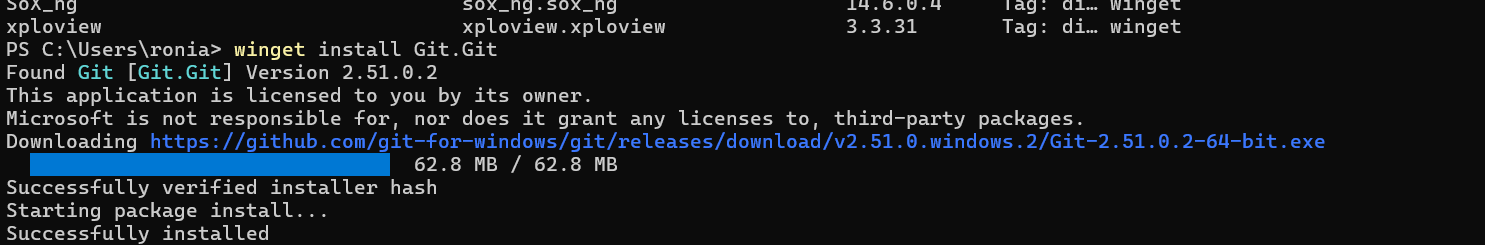
\includegraphics[width=0.9\textwidth]{./assets/images/09_install_git.png}
    \caption{Instalação do Git.}
    \label{fig:install_git}
  \end{figure}
  \item Verifique a instalação digitando, em alguns casos o Windows exige que o terminal seja reiniciado para que as variáveis de ambiente adicionadas com a instalação sejam carregadas corretamente:
  \begin{verbatim}
    git --version
  \end{verbatim}
  O comando deve retornar a versão do Git instalada.
  \begin{figure}[H]
    \centering
    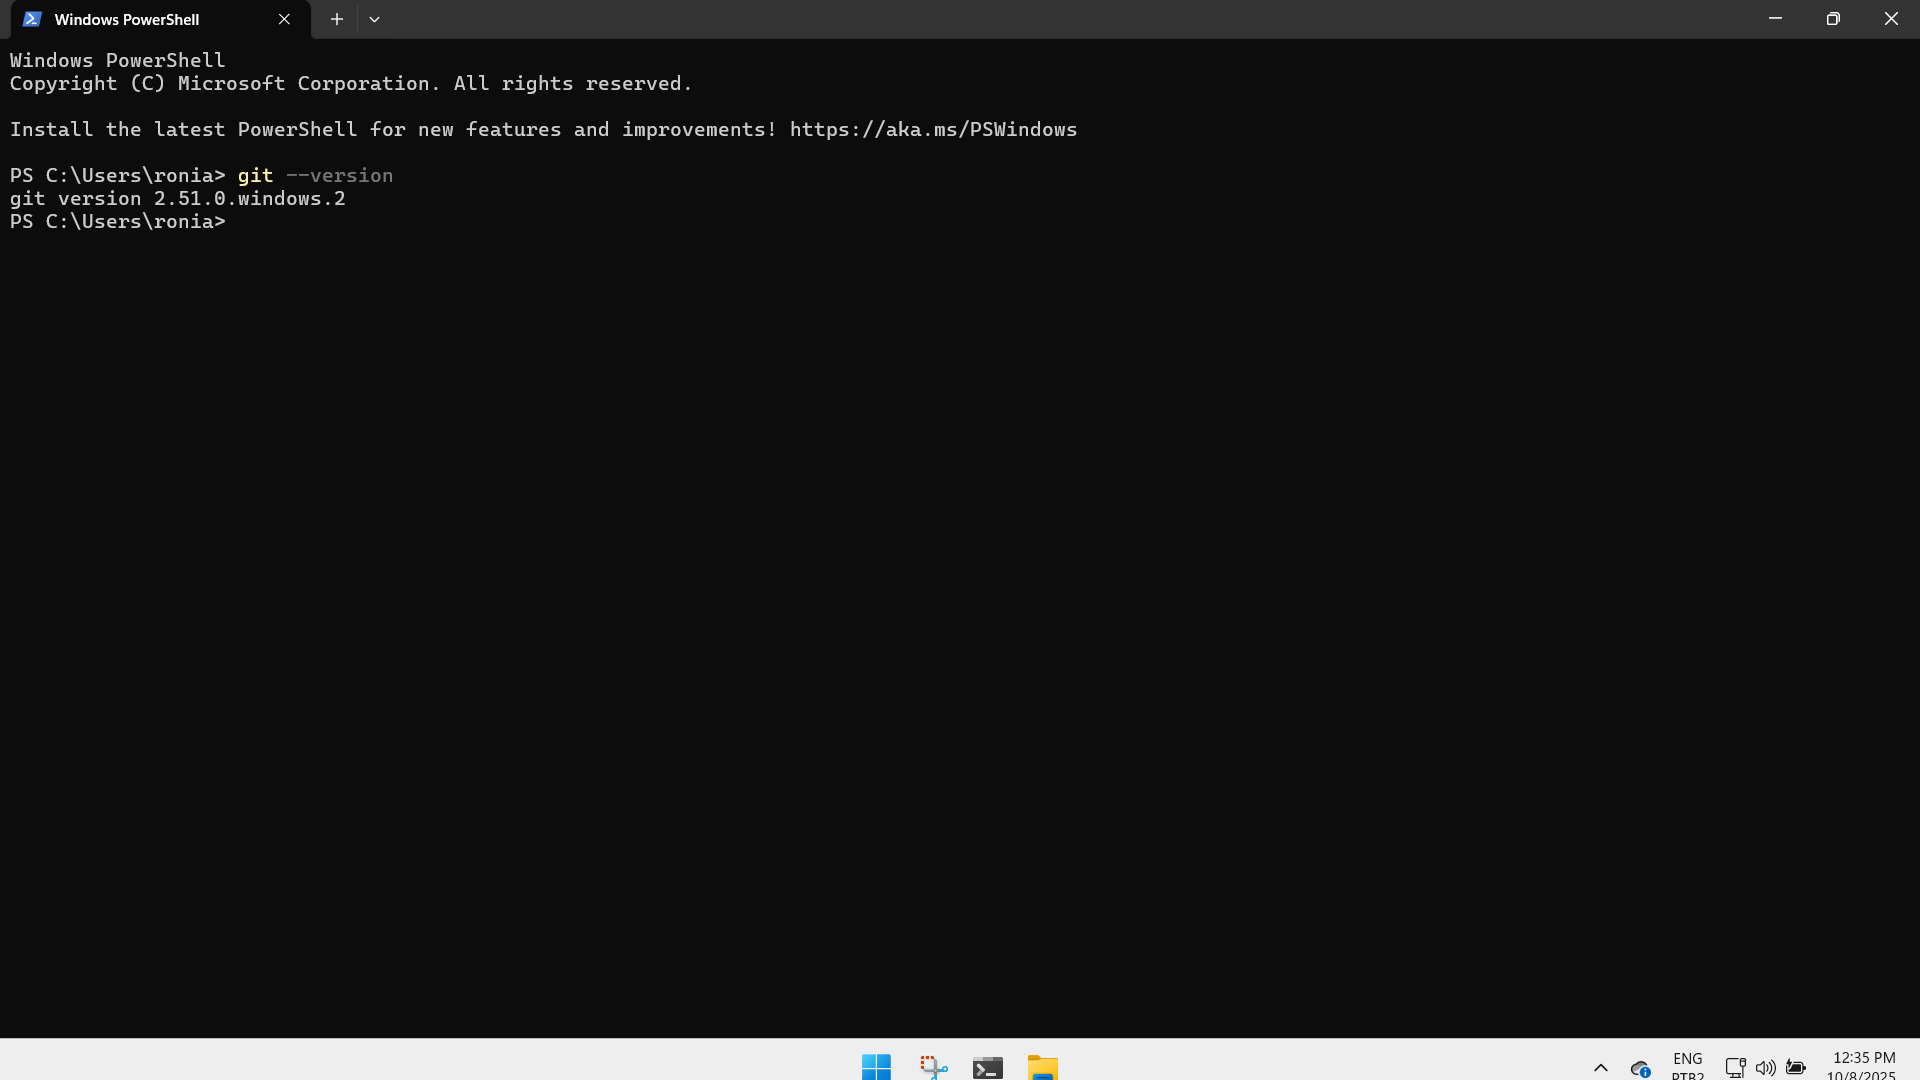
\includegraphics[width=0.9\textwidth]{./assets/images/10_git_version.png}
    \caption{Verificando se o Git está instalado.}
    \label{fig:git_version}
  \end{figure}
\end{enumerate}
\par
\section{O que é o GitHub-CLI?}
O GitHub-CLI (Command Line Interface) é uma ferramenta de linha de comando desenvolvida pela GitHub, Inc., que permite interagir com os repositórios e recursos do GitHub diretamente pelo terminal, sem a necessidade de acessar a interface web.

Com o GitHub-CLI, é possível executar operações comuns como clonar repositórios, criar issues, abrir e revisar pull requests, gerenciar branches, autenticar usuários, visualizar status de workflows e automatizar fluxos de trabalho, integrando-se perfeitamente com o Git e com scripts de automação.

Essa ferramenta é especialmente útil para desenvolvedores que preferem trabalhar no terminal, proporcionando agilidade, automação e maior produtividade no gerenciamento de projetos hospedados no GitHub.
\subsection{Instalação do GitHub-CLI}
\begin{enumerate}
  \item Abra o Prompt de Comando ou PowerShell.
  \item Agora \textcolor{cyan}{id} = \textcolor{cyan}{GitHub.cli}, e digite o comando:
  \begin{verbatim}
    winget install GitHub.cli
  \end{verbatim}
  e pressione Enter.
  \item Aguarde a conclusão da instalação.
  \begin{figure}[H]
    \centering
    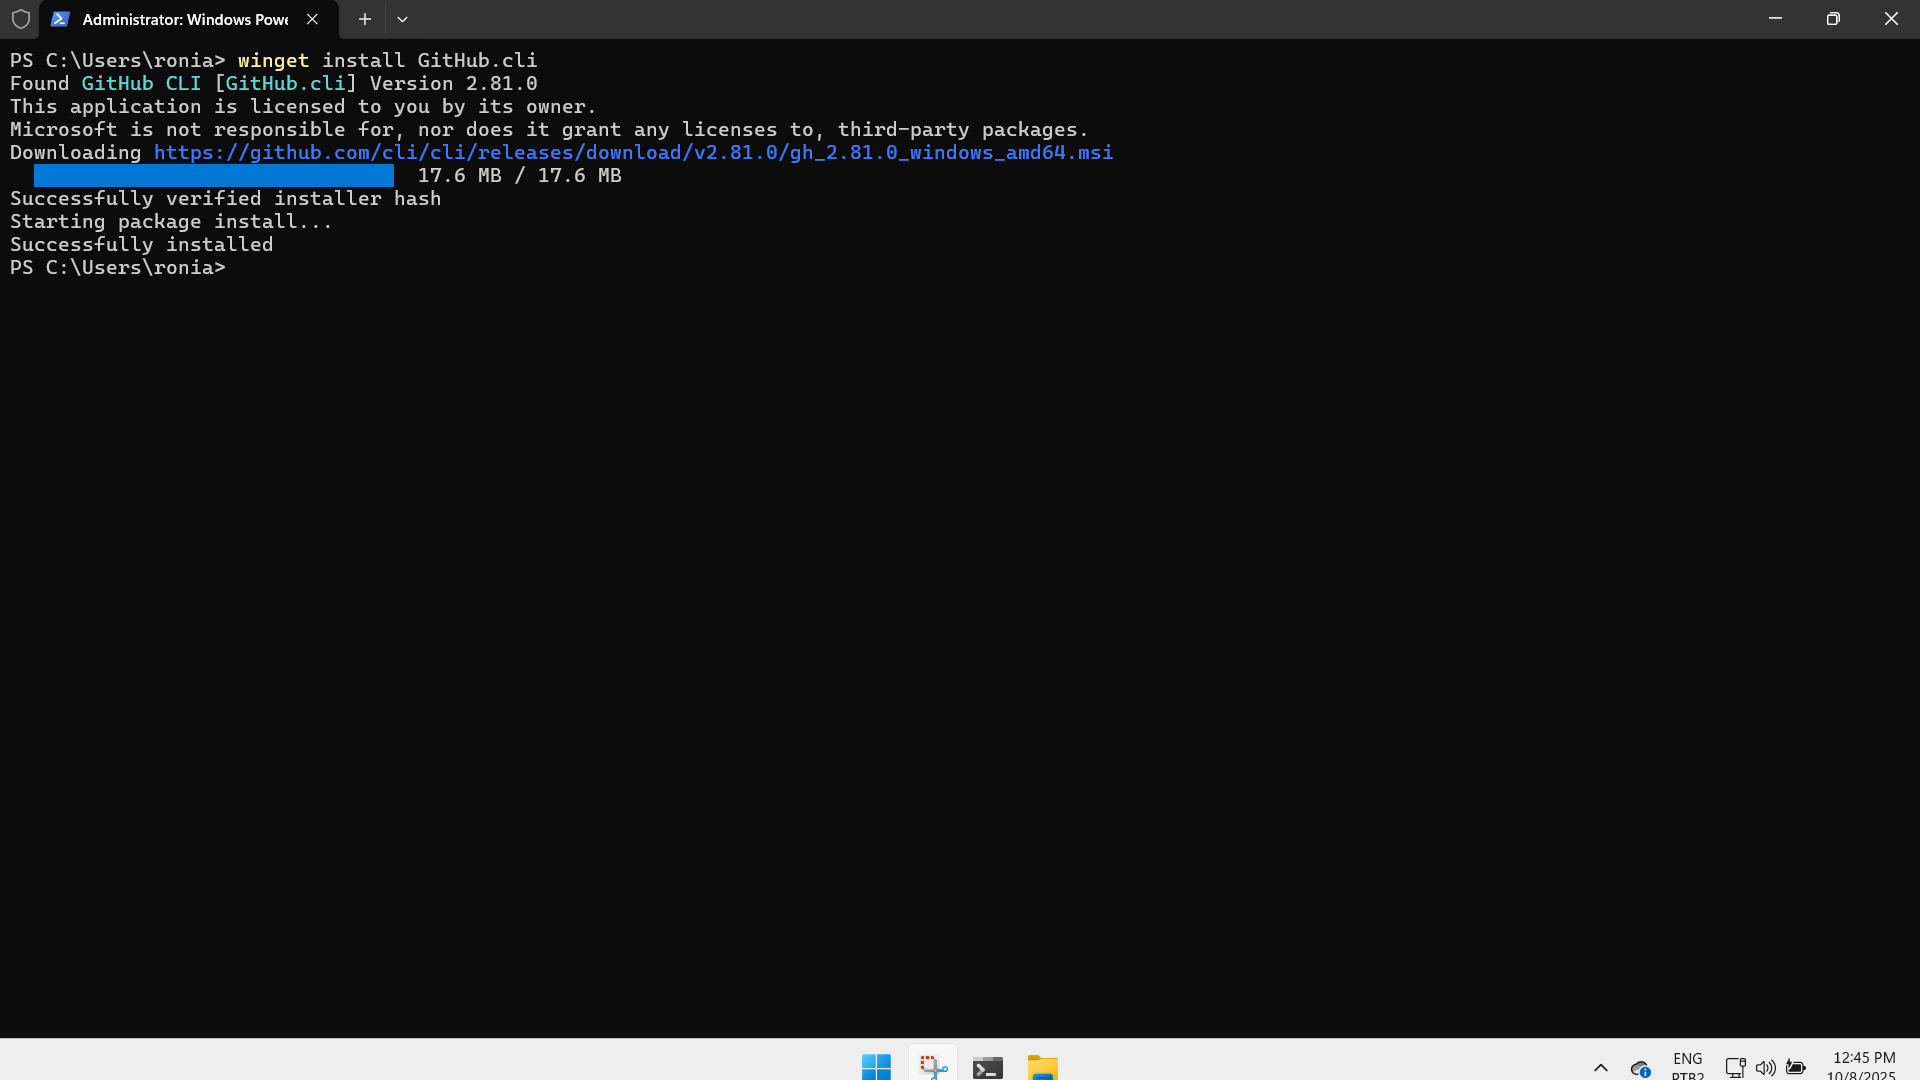
\includegraphics[width=0.9\textwidth]{./assets/images/11_install_cli.png}
    \caption{Instalando o GitHub-CLI.}
    \label{fig:install_cli}
  \end{figure}
  \item Verifique a instalação digitando:
  \begin{verbatim}
    gh --version
  \end{verbatim}
    O comando deve retornar a versão do GitHub-CLI instalada.
    \begin{figure}[H]
    \centering
    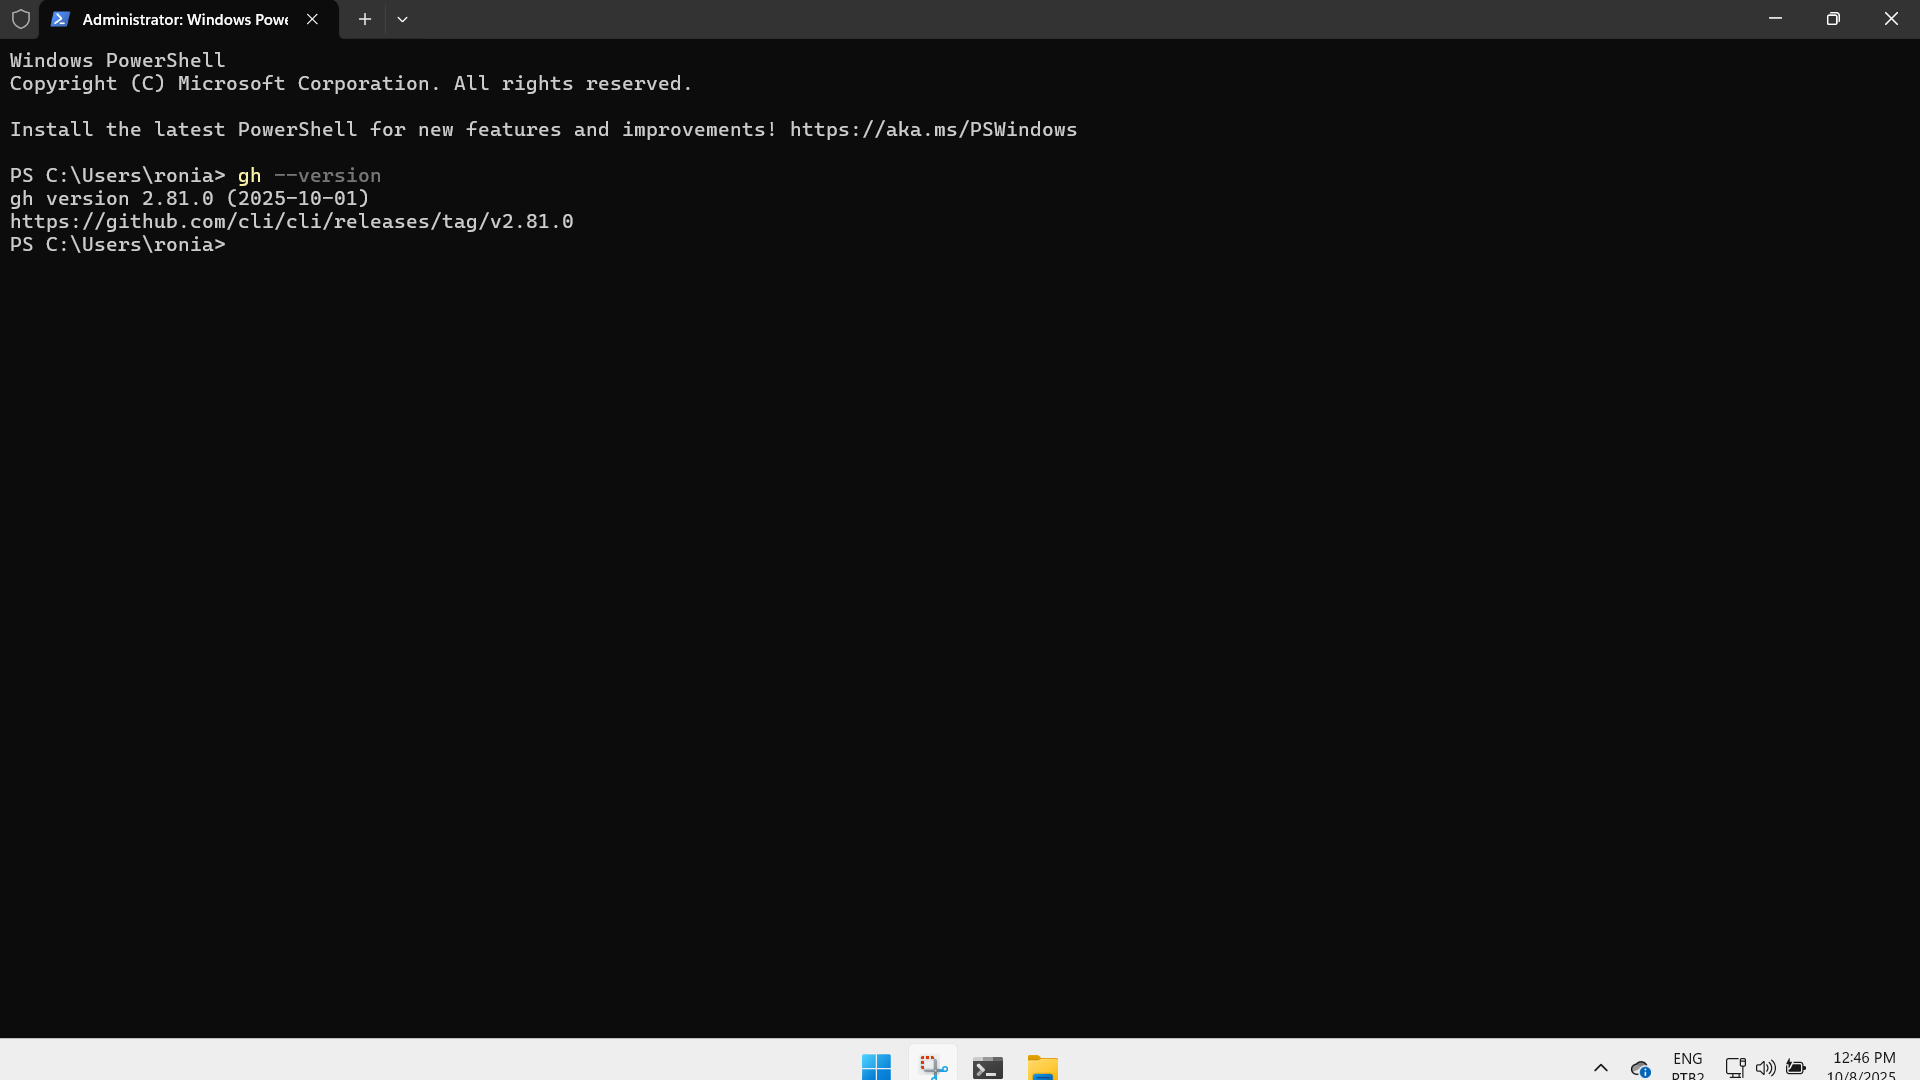
\includegraphics[width=0.9\textwidth]{./assets/images/12_cli_version.png}
    \caption{Verificando se o GitHub-CLI está instalado.}
    \label{fig:cli_version}
  \end{figure}
\end{enumerate}
\par
\section{Configuração do Git e GitHub-CLI}
Após a instalação do Git e do GitHub-CLI, é necessário realizar algumas configurações iniciais para garantir que suas informações estejam corretas ao fazer commits e interagir com o GitHub.
\par
\subsection{Autenticação}
Existem duas formas seguras de autenticação para o Git, a primeira envolve a geração de um token de acesso pessoal (PAT - Personal Access Token) no GitHub, que é usado como senha ao fazer push ou pull de repositórios remotos. A segunda forma é a autenticação via SSH, que envolve a criação de um par de chaves SSH (pública e privada) e a adição da chave pública à sua conta do GitHub. A autenticação via SSH é geralmente mais segura e conveniente, pois elimina a necessidade de inserir o token ou senha repetidamente.

OBS.: \textbf{Desde agosto de 2021, o GitHub não aceita mais autenticação via senha para operações Git que envolvem repositórios remotos. Portanto, é obrigatório o uso de tokens de acesso pessoal (PAT) ou autenticação via SSH para essas operações.}

A opção dois é usando o GitHub-CLI, que facilita o processo de autenticação. A seguir, estão os passos para configurar a autenticação usando o GitHub-CLI.
\par
\subsubsection{Autenticação com o GitHub-CLI}
Para autenticar-se no GitHub-CLI, execute o comando:
\begin{verbatim}
  gh auth login
\end{verbatim}
Siga as instruções na tela para concluir o processo de autenticação.
\begin{figure}[H]
  \centering
  \caption{Efetuando a autenticação com o GitHub-CLI - Passo 1.}
  \label{fig:gh_auth_login_0}
  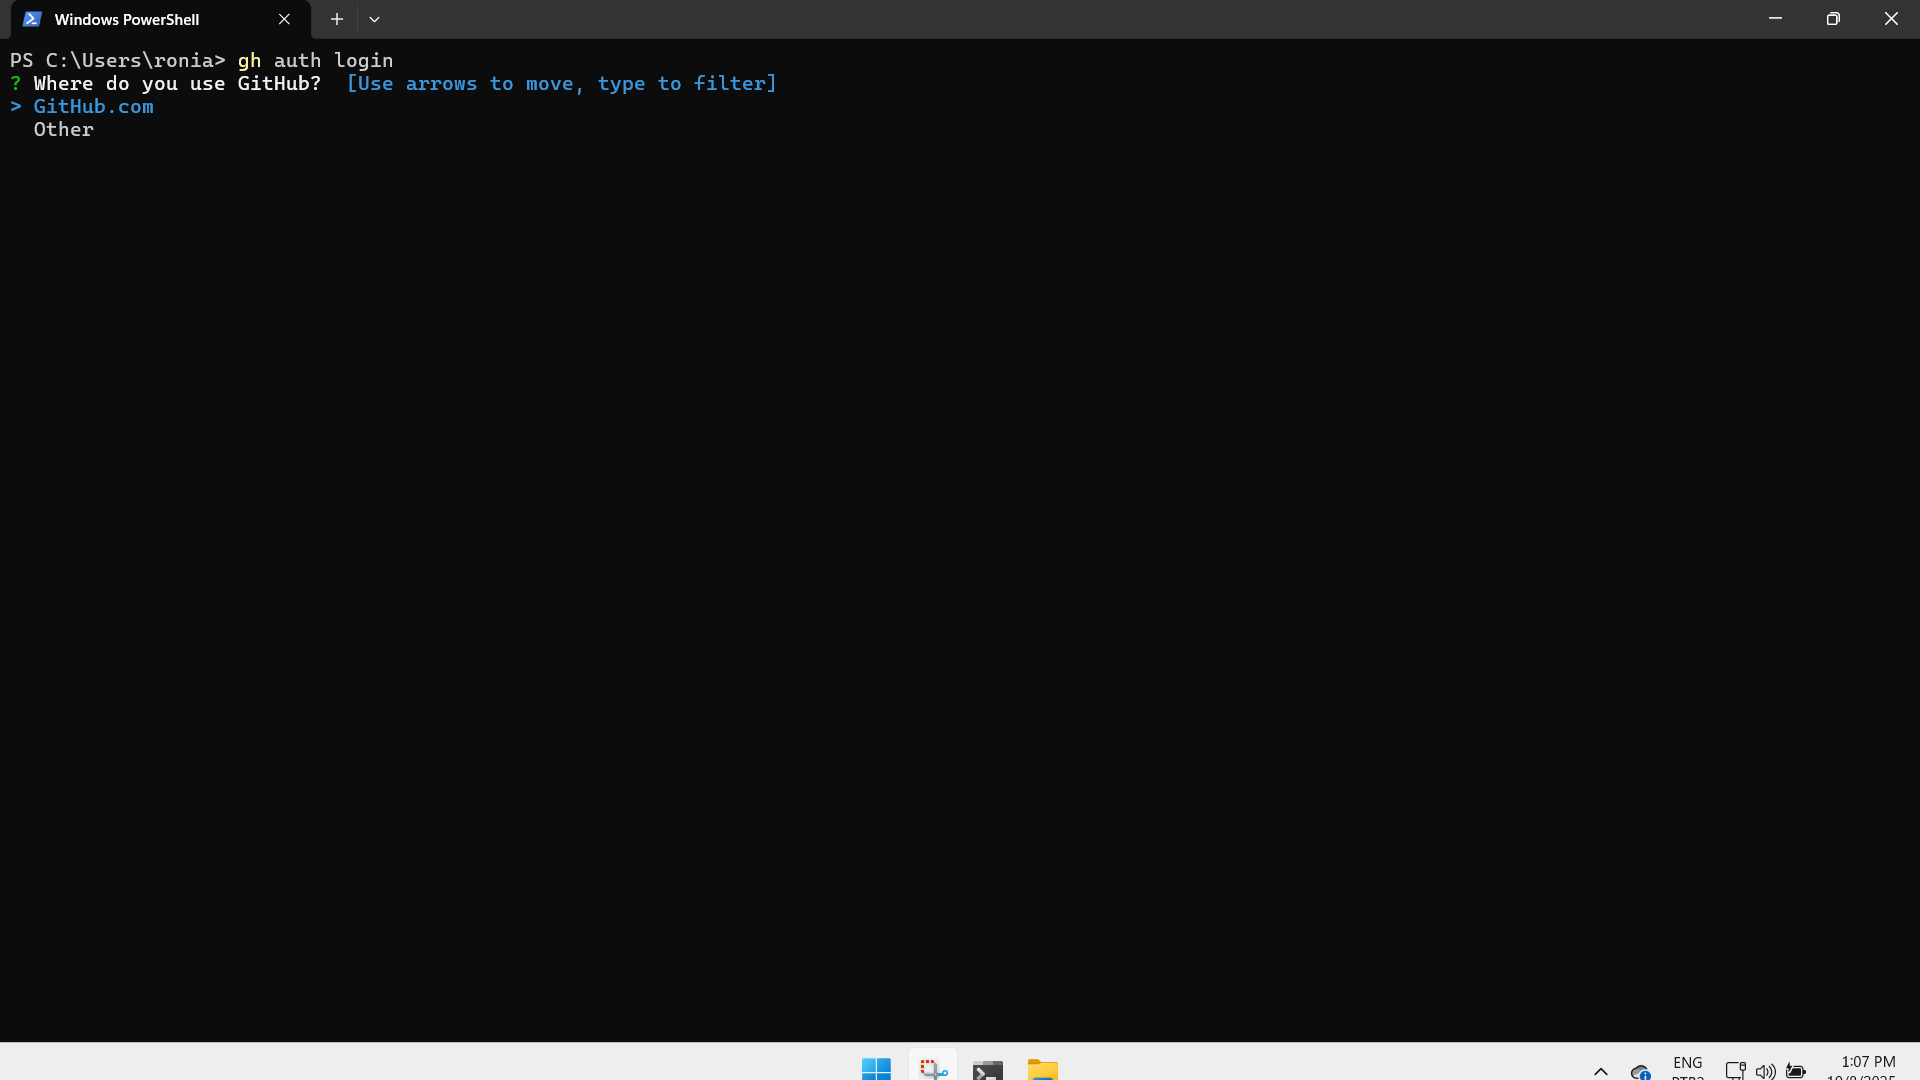
\includegraphics[width=0.9\textwidth]{./assets/images/13_0_gh_auth_login.png}
  \caption{Efetuando a autenticação com o GitHub-CLI - Passo 2.}
  \label{fig:gh_auth_login_1}
  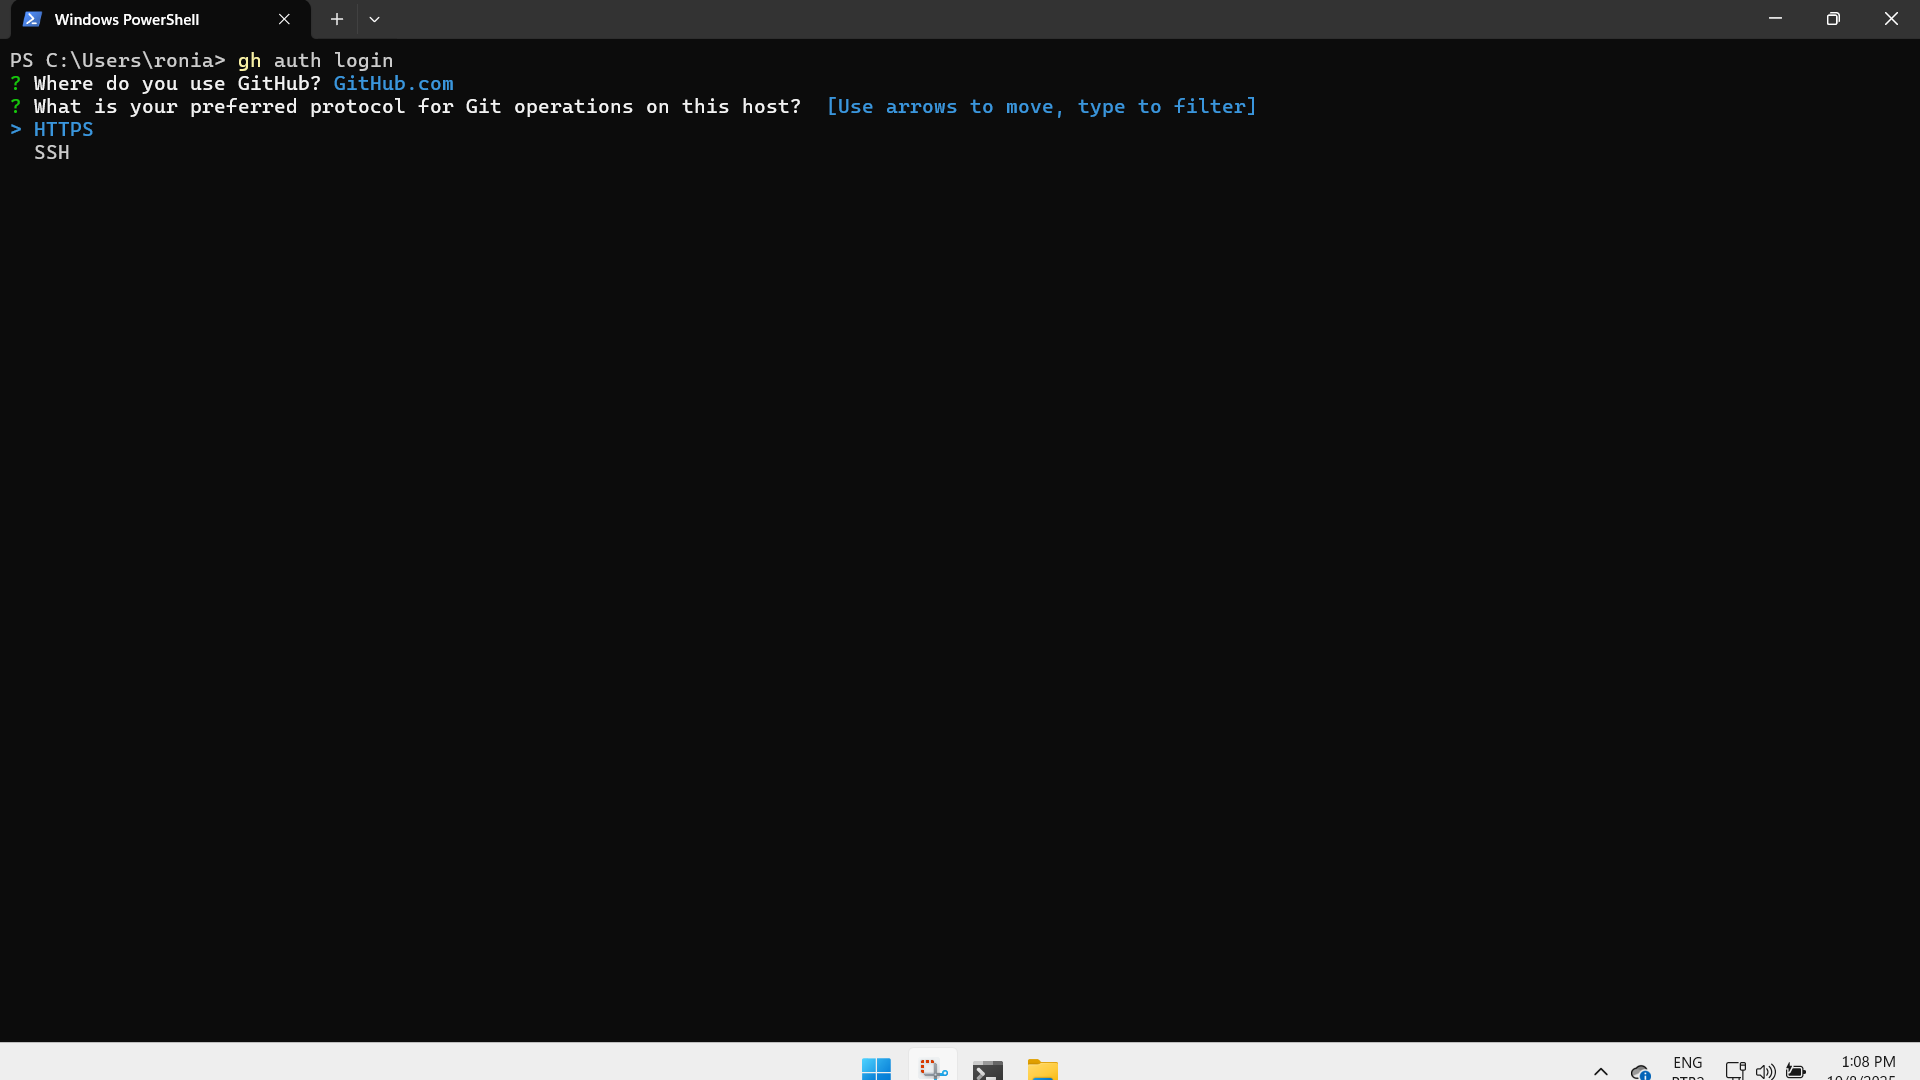
\includegraphics[width=0.9\textwidth]{./assets/images/13_1_gh_auth_login.png}
  \caption{Efetuando a autenticação com o GitHub-CLI - Passo 3.}
  \label{fig:gh_auth_login_2}
  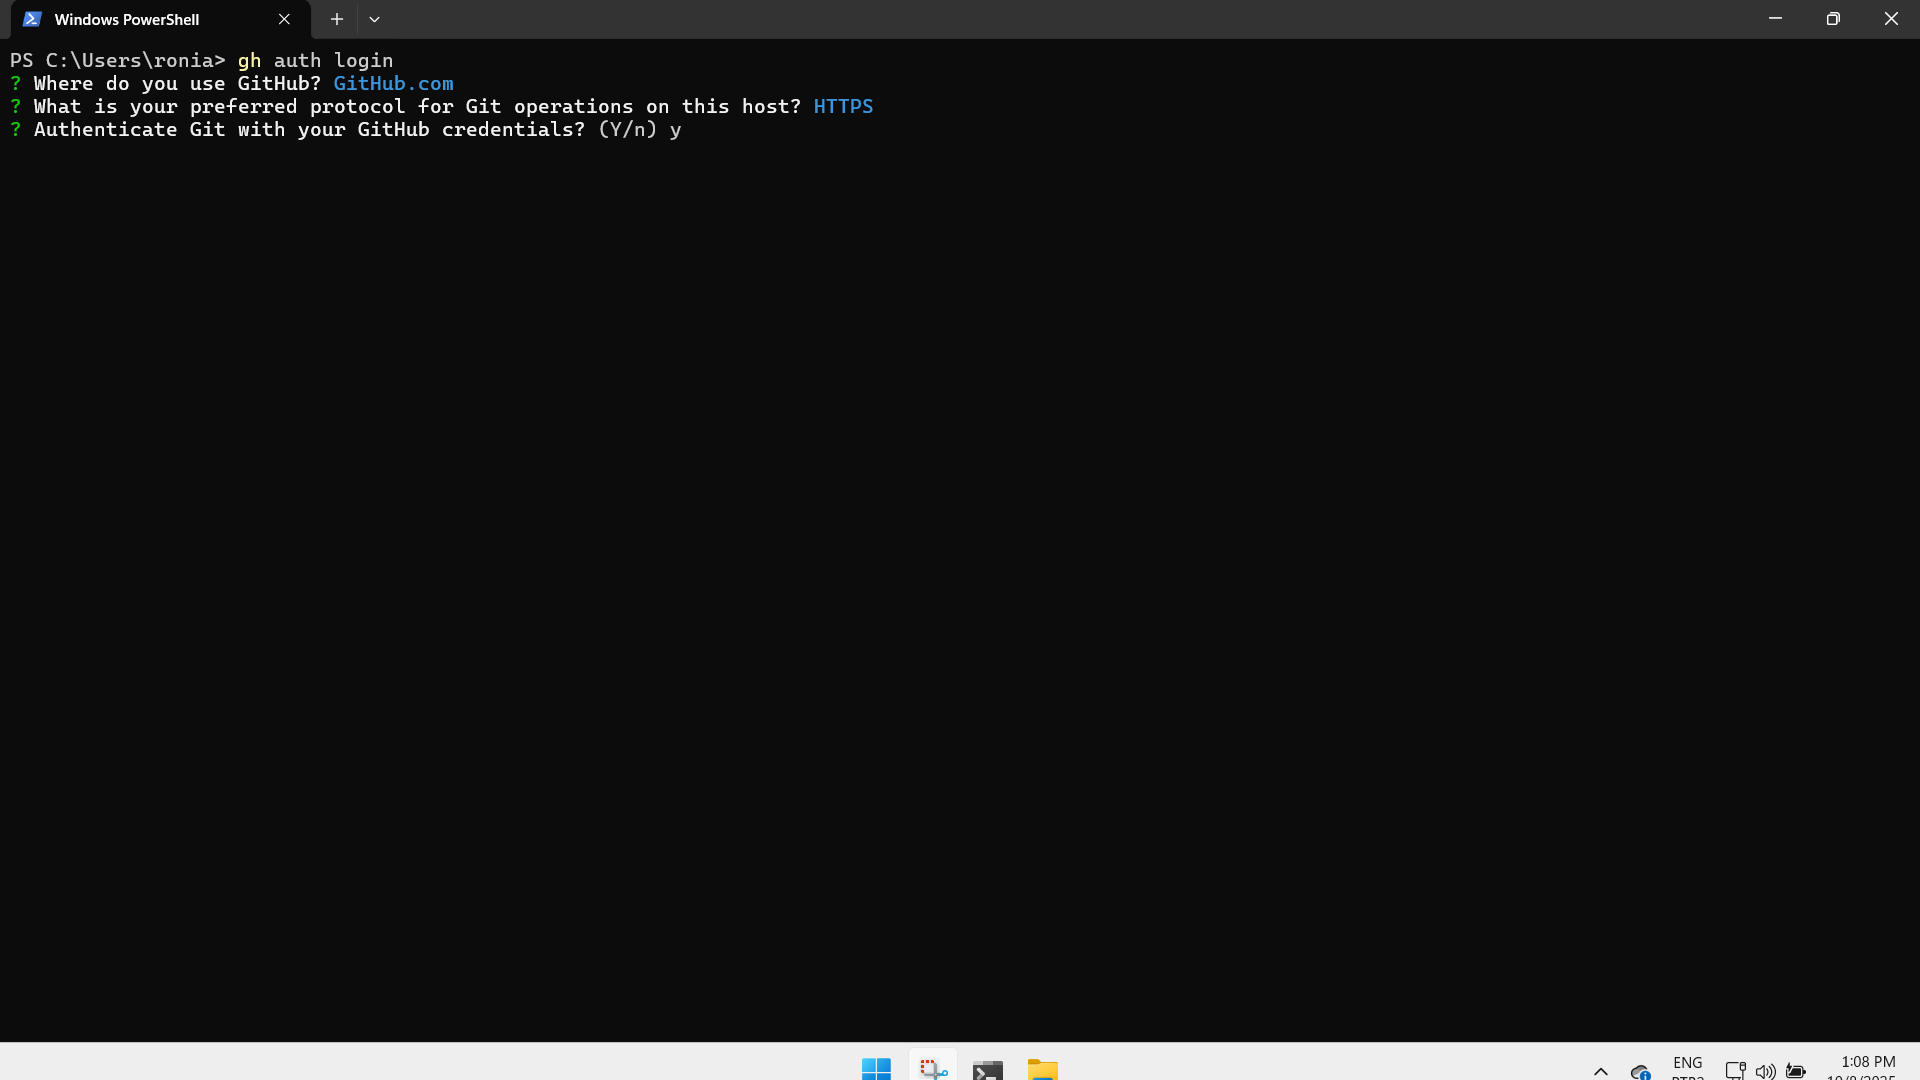
\includegraphics[width=0.9\textwidth]{./assets/images/13_2_gh_auth_login.png}
\end{figure}
\begin{figure}[H]
  \centering
  \caption{Efetuando a autenticação com o GitHub-CLI - Passo 4.}
  \label{fig:gh_auth_login_3}
  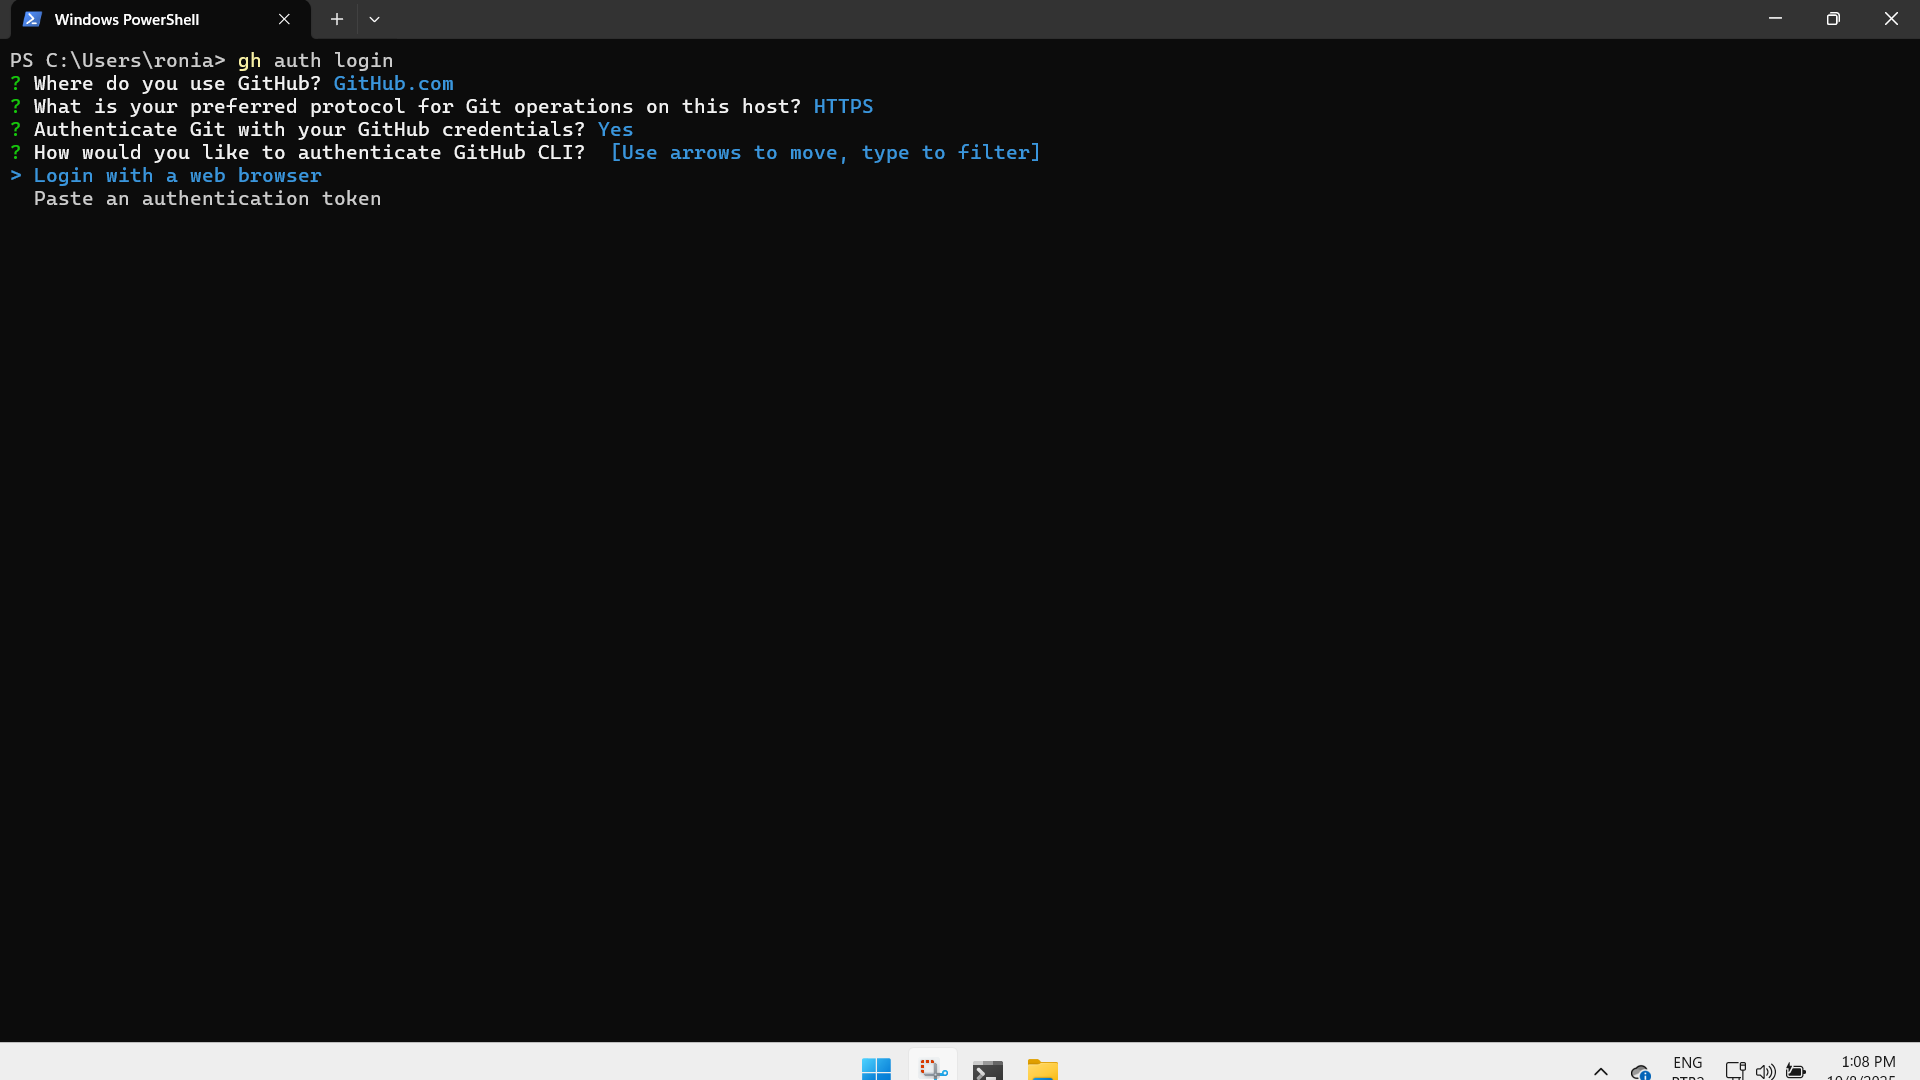
\includegraphics[width=0.9\textwidth]{./assets/images/13_3_gh_auth_login.png}
  \caption{Efetuando a autenticação com o GitHub-CLI - Passo 5.}
  \label{fig:gh_auth_login_4}
  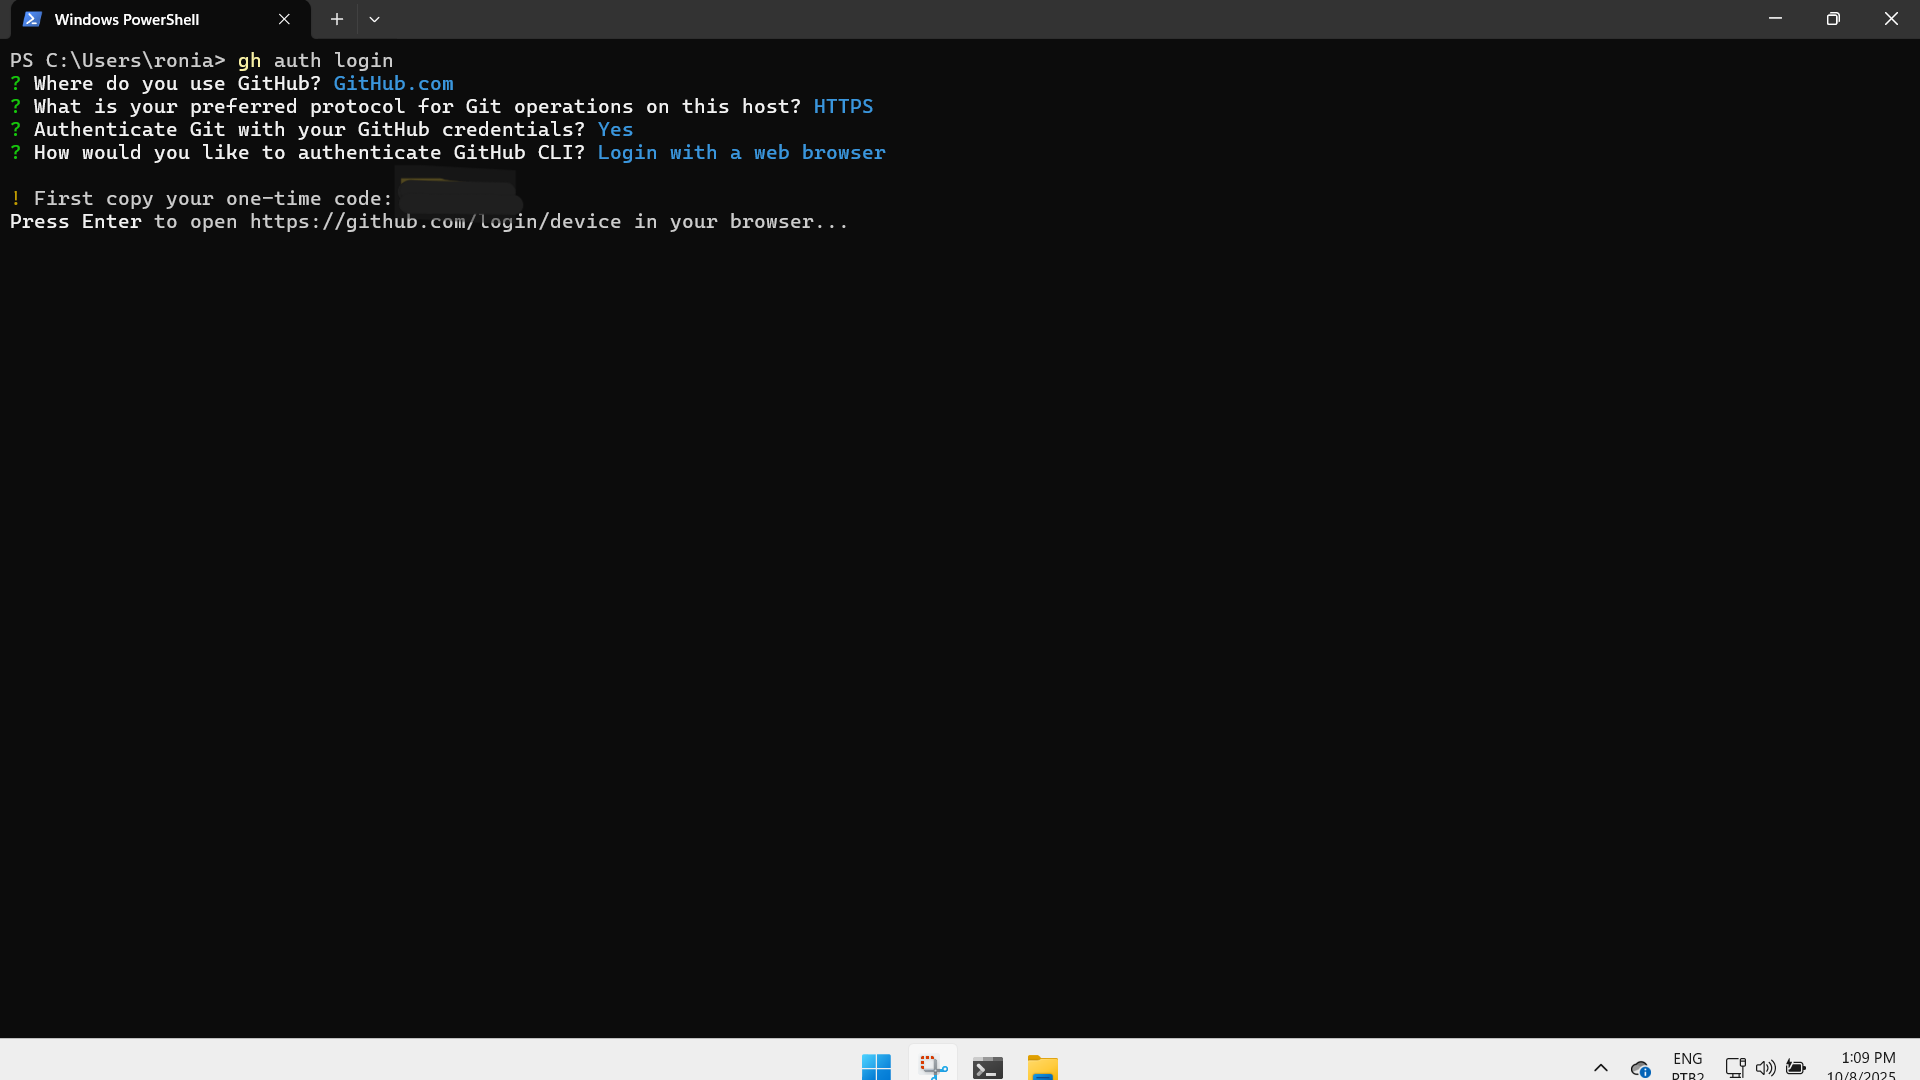
\includegraphics[width=0.9\textwidth]{./assets/images/13_4_gh_auth_login.png}
\end{figure}
\par
Após o passo 5 na Figura \ref{fig:gh_auth_login_4}, p.\pageref{fig:gh_auth_login_4}, será preciso copiar o código gerado abrir o navegador no link fornecido ou se precionar a tecla \texttt{Enter} abrirá o link automaticamente. Nessa tela será pedido que você se autentique e em seguida aparecerá o campo para digitar o código gerado e algumas permissões serão solicitadas.
\subsection{Configuração de usuário Git}
\begin{enumerate}
  \item Abra o Prompt de Comando ou PowerShell.
  \item Verifique a instalação do Git digitando:
  \begin{verbatim}
    git --version
  \end{verbatim}
  O comando deve retornar a versão do Git instalada.
  \item Configure seu nome de usuário com o comando:
  \begin{verbatim}
    git config --global user.name "Seu Nome"
  \end{verbatim}
  Substitua "Seu Nome" pelo nome que você deseja associar aos seus commits e pressione Enter.
  \item Verifique se o nome foi configurado corretamente com o comando:
  \begin{verbatim}
    git config --global user.name
  \end{verbatim}
  Pressione Enter.
  O comando deve retornar o nome que você configurou.
  \item Agora, configure seu e-mail com o comando:
  \begin{verbatim}
    git config --global user.email "Seu E-mail"
  \end{verbatim}
  Substitua "Seu E-mail" pelo e-mail que você deseja associar aos seus commits e pressione Enter.
  \item Verifique se o e-mail foi configurado corretamente com o comando:
  \begin{verbatim}
    git config --global user.email
  \end{verbatim}
  Pressione Enter.
  O comando deve retornar o e-mail que você configurou.
  \begin{figure}[H]
    \centering
    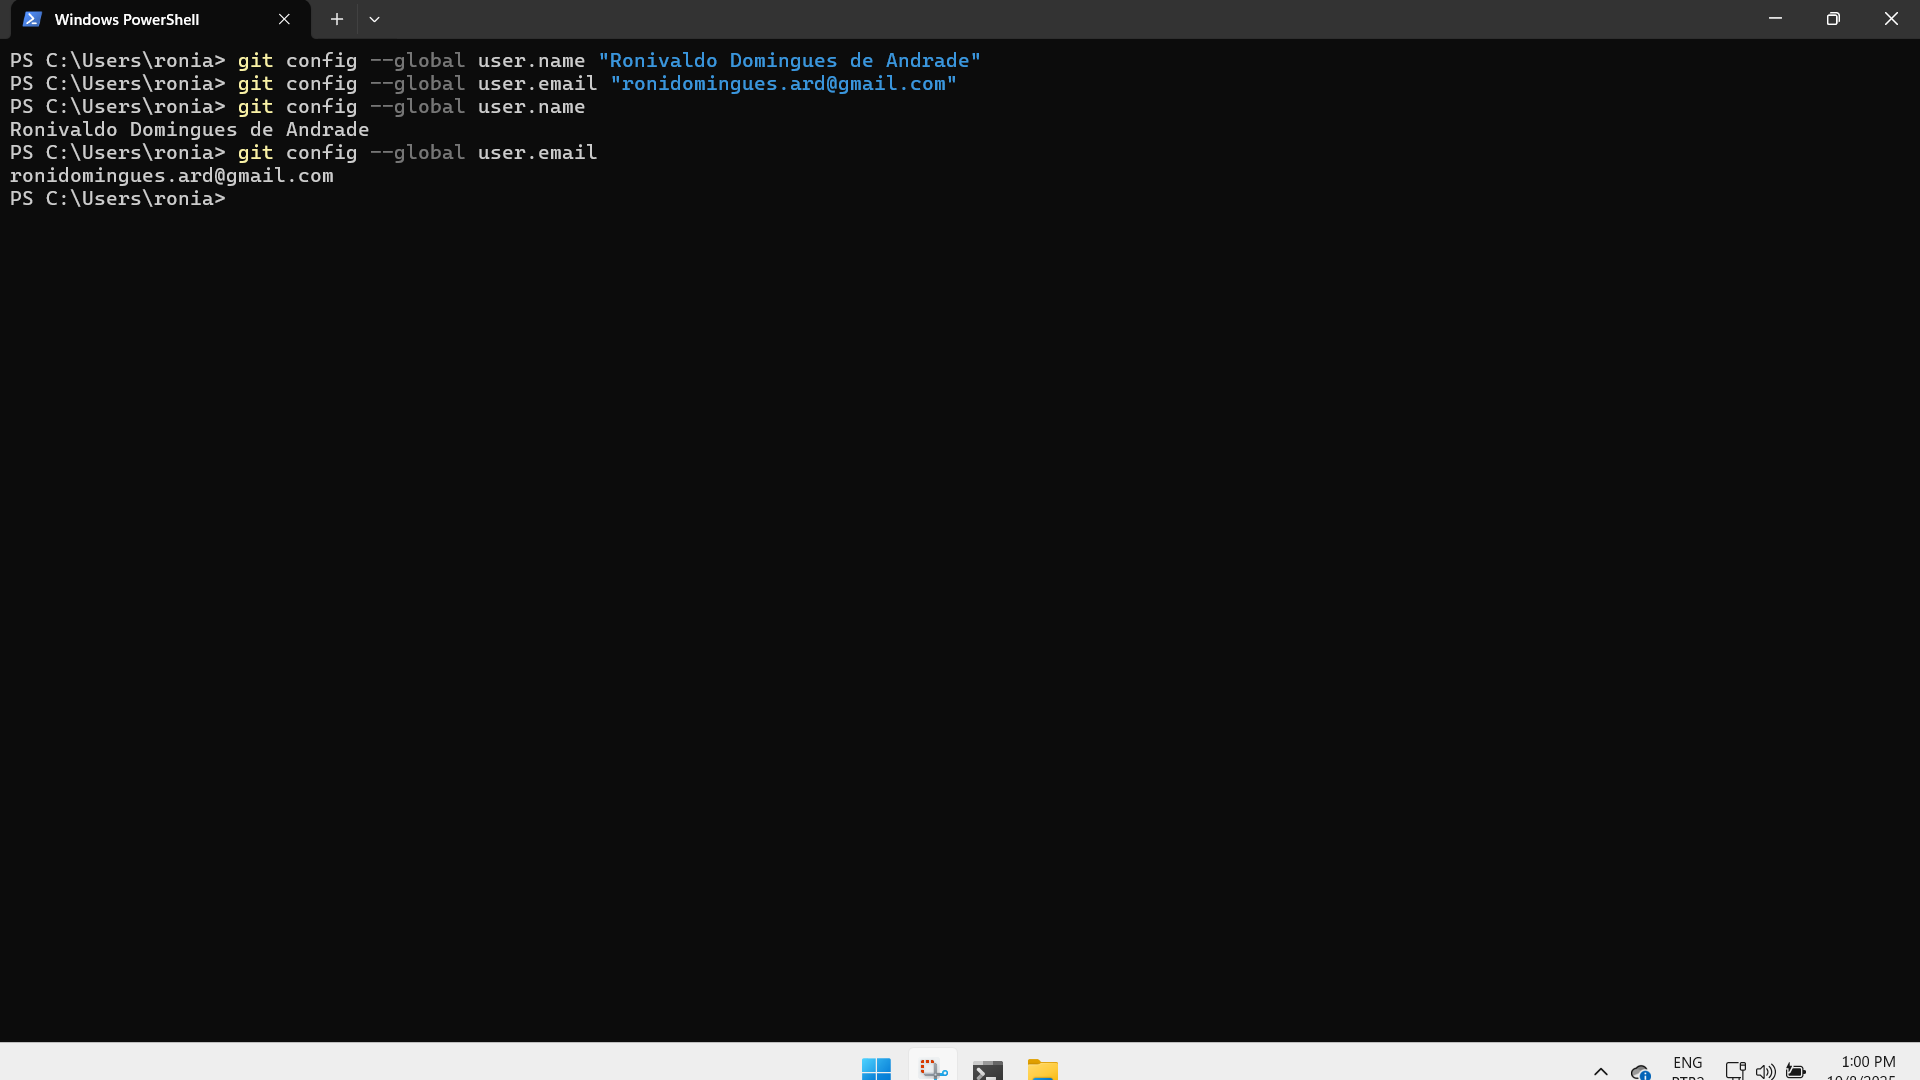
\includegraphics[width=0.9\textwidth]{./assets/images/14_git_base_config.png}
    \caption{Configurando o Git.}
    \label{fig:git_base_config}
  \end{figure}
\end{enumerate}
\par
\subsubsection{Autenticação usando PAT (Opcional)}
O uso da autenticação com Personal Access Token (PAT) no GitHub oferece maior segurança em comparação à utilização de senhas tradicionais. Isso porque o token pode ser revogado a qualquer momento diretamente nas configurações da conta, além de possuir um prazo de validade configurável no momento da criação.
Ademais, os PATs permitem definir escopos específicos de acesso, garantindo que o token tenha apenas as permissões necessárias para a operação desejada.
Se você optar por usar um Token de Acesso Pessoal (PAT) para autenticação, siga os passos abaixo:
\begin{enumerate}
  \item Acesse o link \url{https://github.com/settings/tokens} na sua conta do GitHub.
  \item Clique em "Generate new token (classic)".
  \item Marque escopos como:
  \begin{itemize}
    \item repo (para acesso completo a repositórios privados e públicos)
    \item  workflows (para gerenciar e visualizar GitHub Actions)
  \end{itemize}
  \item Clique em "Generate token" na parte inferior da página e copie o token gerado (ele não será mostrado novamente!).
  \item Agora, ao fazer um git push, quando o Git solicitar senha e usuario:
  \begin{itemize}
    \item Use seu nome de usuário do GitHub como usuário.
    \item Cole o token gerado como senha.
  \end{itemize}
  \item Você também pode salvar o token gerado no cache de credenciais do Git para evitar ter que digitá-lo toda vez que fizer push ou pull. Para isso, use o comando:
  \begin{verbatim}
    git config --global credential.helper store
  \end{verbatim}
  Com isso, na próxima vez que você digitar o token, ele será salvo no arquivo `~/.git-credentials` e usado automaticamente nas próximas operações.
\end{enumerate}
\par
\subsection{Configuração de Editor Padrão (Opcional)}
Você pode configurar o editor de texto padrão que será usado para escrever mensagens de commit. Por exemplo, para configurar o Visual Studio Code como editor padrão, use o comando:
\begin{verbatim}
  git config --global core.editor "code --wait"
\end{verbatim}
Substitua "code --wait" pelo comando do editor de sua preferência.
\par
\subsection{Configurar a branch padrão para 'main' (Opcional)}
Para configurar a branch padrão para 'main', use o comando:
\begin{verbatim}
  git config --global init.defaultBranch main
\end{verbatim}
Isso garantirá que novos repositórios criados localmente usem 'main' como a branch padrão. Caso não queira definir esse padrão é possivel mudar a branch individualmente para cada repositório com o comando:
\begin{verbatim}
  git branch -M main
\end{verbatim}
\par
Obs.: \textbf{A partir de outubro de 2020, o GitHub alterou o nome da branch padrão de "master" para "main" em novos repositórios. Portanto, é recomendável usar "main" como a branch padrão para novos projetos.}
\par
\section{Comandos Básicos do Git e GitHub-CLI}
Aqui estão alguns comandos básicos do Git e do GitHub-CLI que você deve conhecer para começar a trabalhar com repositórios no GitHub.
\par
\subsection{Comandos Básicos do Git}
\begin{itemize}
  \item \textbf{git init}: Inicializa um novo repositório Git local.
  \item \textbf{git clone <url>}: Clona um repositório remoto para o seu computador.
  \item \textbf{git status}: Exibe o status atual do repositório, mostrando arquivos modificados, não rastreados e prontos para commit.
  \item \textbf{git add <arquivo>}: Adiciona um arquivo específico ao estágio para commit.
  \item \textbf{git add .}: Adiciona todos os arquivos modificados ao estágio para commit.
  \item \textbf{git commit -m "mensagem"}: Cria um commit com uma mensagem descritiva.
  \item \textbf{git push}: Envia os commits locais para o repositório remoto.
  \item \textbf{git pull}: Puxa as alterações do repositório remoto para o repositório local.
  \item \textbf{git branch}: Lista todas as branches no repositório.
  \item \textbf{git checkout <branch>}: Muda para a branch especificada.
  \item \textbf{git branch -M <branch>}: Renomeia a branch atual para o nome especificado forçando a sobrescrita se a branch especificada já existir.
  \item \textbf{git branch -m <branch>}: Renomeia a branch atual para o nome especificado e falha se a branch especificada já existir.
  \item \textbf{git checkout -b <branch>}: Cria uma nova branch e muda para ela.
  \item \textbf{git branch -d <branch>}: Deleta a branch especificada.
  \item \textbf{git remote rm origin}: Remove o repositório remoto chamado "origin".
  \item \textbf{git remote add origin <url>}: Adiciona um repositório remoto com o nome "origin".
  \item \textbf{git remote -v}: Exibe os repositórios remotos configurados.
  \item \textbf{git merge <branch>}: Mescla a branch especificada na branch atual.
  \item \textbf{Veja mais comandos do Git na tabela \ref{tab:gitcommands}, p.\pageref{tab:gitcommands}.}
\end{itemize}
\par
\subsection{Comandos Básicos do GitHub-CLI}
\begin{itemize}
  \item \textbf{gh auth login}: Autentica o usuário no GitHub-CLI.
  \item \textbf{gh repo create <nome-do-repositorio>}: Cria um novo repositório no GitHub.
  \item \textbf{gh repo clone <nome-do-repositorio>}: Clona um repositório do GitHub para o seu computador.
  \item \textbf{gh issue create}: Cria uma nova issue no repositório atual.
  \item \textbf{gh pr create}: Cria um novo pull request.
  \item \textbf{gh pr checkout <numero-do-pr>}: Faz checkout de um pull request específico.
  \item \textbf{gh pr merge <numero-do-pr>}: Mescla um pull request específico.
  \item \textbf{gh repo view}: Exibe informações sobre o repositório atual.
  \item \textbf{gh gist create <arquivo>}: Cria um novo gist com o arquivo especificado.
  \item \textbf{Veja mais comandos do GitHub-CLI na tabela \ref{tab:githubcli_commands}, p.\pageref{tab:githubcli_commands}.}
\end{itemize}
\par    % Git e GitHub CLI
\chapter{Git LFS}
\section{O que é?}

O \textbf{Git LFS (Large File Storage)} é uma extensão oficial do Git projetada para o gerenciamento de \textbf{arquivos grandes ou binários} que não são tratados de forma eficiente pelo Git tradicional.  
Em vez de armazenar o conteúdo completo desses arquivos no histórico do repositório, o Git LFS substitui o arquivo original por um \textbf{ponteiro leve} — um pequeno arquivo de texto contendo informações sobre o objeto real, como seu identificador (\textit{hash}) e tamanho.  
O conteúdo real é armazenado separadamente, em um \textbf{servidor LFS}, podendo estar hospedado no próprio provedor Git (como o GitHub, GitLab ou Bitbucket) ou em um servidor dedicado.

Essa estratégia mantém o repositório \textbf{mais leve e ágil}, reduzindo o tempo de \textit{clone}, \textit{checkout} e \textit{fetch}, além de facilitar o versionamento de arquivos que mudam com frequência, como imagens, vídeos, áudios, modelos de aprendizado de máquina, arquivos de design (\texttt{.psd}), pacotes compactados (\texttt{.zip}), entre outros.

\subsection{Motivos e Problemas que Resolve}

Por padrão, o Git não é otimizado para lidar com arquivos grandes ou binários, pois ele foi projetado para versionar \textbf{texto}, como código-fonte.  
Existem várias limitações e problemas ao tentar versionar arquivos grandes diretamente:

\begin{itemize}
  \item \textbf{Limite de tamanho:} serviços como o GitHub impõem limites de \textbf{100 MB por arquivo}, impedindo o envio de arquivos muito grandes via Git comum.
  \item \textbf{Histórico inflado:} cada nova versão de um arquivo binário é armazenada integralmente, sem compressão eficiente, o que faz o repositório crescer rapidamente.
  \item \textbf{Operações lentas:} com muitos arquivos grandes no histórico, operações como \texttt{git clone}, \texttt{git fetch} e \texttt{git checkout} tornam-se mais lentas.
  \item \textbf{Dificuldade de merge:} arquivos binários não podem ser mesclados (\textit{merge}) facilmente, aumentando o risco de conflitos.
\end{itemize}

O \textbf{Git LFS} resolve esses problemas ao:
\begin{itemize}
  \item Armazenar apenas \textbf{ponteiros leves} no repositório Git;
  \item Manter o conteúdo real em um \textbf{armazenamento separado}, acessível sob demanda;
  \item Permitir a \textbf{revogação ou substituição} de arquivos sem reescrever o histórico;
  \item Proporcionar uma experiência de versionamento \textbf{transparente}, pois os comandos Git (\texttt{add}, \texttt{commit}, \texttt{push}) continuam funcionando normalmente.
\end{itemize}

\subsection{Como Funciona}

O Git LFS utiliza um sistema de filtros configurados no Git:
\begin{itemize}
  \item O filtro \textbf{clean} atua ao adicionar um arquivo rastreado pelo LFS, substituindo seu conteúdo real por um ponteiro antes de armazená-lo no repositório.
  \item O filtro \textbf{smudge} atua durante o \texttt{checkout} ou \texttt{clone}, baixando automaticamente o arquivo real do servidor LFS e substituindo o ponteiro pelo conteúdo original no diretório de trabalho.
\end{itemize}

O arquivo versionado no Git contém apenas algo como:

\begin{verbatim}
version https://git-lfs.github.com/spec/v1
oid sha256:3b6f1a8a...
size 1258291
\end{verbatim}

Essas informações são suficientes para que o Git LFS localize e baixe o conteúdo correto quando necessário.

\subsection{Vantagens}

\begin{itemize}
  \item Mantém o repositório leve e rápido;
  \item Suporta arquivos grandes (acima de 100 MB);
  \item Permite versionamento de arquivos binários;
  \item Integra-se com GitHub, GitLab e Bitbucket;
  \item Possibilita bloqueio de arquivos (\textit{lock}) para evitar conflitos.
\end{itemize}

\subsection{Limitações}

\begin{itemize}
  \item O armazenamento LFS pode ter \textbf{cotas e custos adicionais} em serviços remotos;
  \item Necessita de \textbf{instalação e configuração} local (\texttt{git lfs install});
  \item Requer que o \textbf{servidor remoto suporte LFS};
  \item Para repositórios antigos, pode ser necessário \textbf{migrar o histórico}.
\end{itemize}

\subsection{Exemplo de Uso}

\begin{verbatim}
# Instala o Git LFS no sistema
git lfs install

# Define tipos de arquivo que serão rastreados pelo LFS
git lfs track "*.zip"
git lfs track "*.psd"

# Adiciona e versiona normalmente
git add .gitattributes
git add arquivo.zip
git commit -m "Adiciona arquivo grande com Git LFS"
git push origin main
\end{verbatim}

\subsection{Boas Práticas}

\begin{itemize}
  \item Configure o Git LFS \textbf{antes de adicionar arquivos grandes};
  \item Use o comando \texttt{git lfs track} para definir padrões de arquivos;
  \item Verifique o status com \texttt{git lfs status};
  \item Evite rastrear arquivos pequenos em grande quantidade;
  \item Monitore o uso de armazenamento e transferências.
\end{itemize}    % Repositórios
\chapter{Commits, Merges e Pull Requests}

\section{Introdução}
Commits, merges e pull requests são elementos centrais no fluxo de trabalho com Git e plataformas como GitHub.  
Um \textbf{commit} é uma unidade lógica de alteração no repositório; um \textbf{merge} integra mudanças de uma branch em outra; e um \textbf{pull request} (PR) é uma solicitação formal de revisão e integração de uma branch — normalmente usada em colaboração para revisar código, executar checks automáticos (CI) e registrar a decisão de integrar.

\section{Commits}

\subsection{O que é um commit}
Um commit registra o estado do diretório de trabalho (os arquivos staged) em um nó do histórico do Git. Cada commit tem um identificador (SHA), metadata (autor, data) e uma mensagem que descreve a mudança.

\subsection{Boas práticas de commits}
\begin{itemize}
  \item Faça commits atômicos: cada commit deve representar uma \emph{única} mudança lógica.  
  \item Mensagens claras: use assunto imperativo curto (\(\sim\)50 caracteres) + linha em branco + corpo explicativo se necessário (72 caracteres por linha).  
  \item Inclua referência a issues quando relevante (ex.: ``Closes \#42'').  
  \item Evite commitar arquivos gerados (binários, dependências) — use \texttt{.gitignore}.  
  \item Assine commits quando necessário: \texttt{git commit -S -m "..."} (GPG).
\end{itemize}

\subsection{Fazendo commits — passo a passo}
\begin{enumerate}
  \item Verificar o estado dos arquivos:
  \begin{verbatim}
  git status
  \end{verbatim}
  \item Ver as mudanças não staged:
  \begin{verbatim}
  git diff       # diferenças não adicionadas ao stage
  git diff --staged  # diferenças preparadas para commit
  \end{verbatim}
  \item Adicionar alterações ao stage (todo arquivo ou interativo):
  \begin{verbatim}
  git add caminho/arquivo.txt  # adiciona arquivo específico
  git add .                    # adiciona tudo (cuidado)
  git add -p                   # adiciona parcialmente (patch)
  \end{verbatim}
  \item Criar o commit com boa mensagem:
  \begin{verbatim}
  git commit -m "Assunto curto em imperativo"
  # ou para mensagem longa (editor):
  git commit
  \end{verbatim}
  Exemplo de mensagem:
  \begin{verbatim}
  Corrige cálculo de juros

  Ajusta a fórmula de cálculo para considerar juros compostos
  quando o período é maior que 12 meses. Testes unitários
  adicionados para cobrir casos de fronteira.
  \end{verbatim}
  \item Ver histórico resumido:
  \begin{verbatim}
  git log --oneline --graph --decorate --all
  \end{verbatim}
\end{enumerate}

\subsection{Editar o último commit / corrigir mensagens}
\begin{verbatim}
# alterar o conteúdo do último commit (já staged)
git commit --amend

# alterar apenas a mensagem do último commit
git commit --amend -m "Nova mensagem"
\end{verbatim}
\textbf{Atenção:} se o commit já foi enviado ao remoto, evite \texttt{--amend} sem combinar com a equipe — ele reescreve o histórico e exigirá push forçado.

\subsection{Desfazer / alterar staging}
\begin{verbatim}
git restore --staged arquivo.txt   # remove do stage, mantém
                                   # alteração no working tree

git restore arquivo.txt            # descarta alteração no
                                   # working tree (se não commitada)

git reset --soft HEAD~1            # desfaz último commit, mantendo
                                   # mudanças staged

git reset --mixed HEAD~1           # desfaz último commit, mantendo
                                   # mudanças no working tree
                                   # (unstaged)

git reset --hard HEAD~1            # desfaz último commit e 
                                   # descarta mudanças (CUIDADO)
\end{verbatim}

\subsection{Padrões de Commits}

Manter um padrão consistente nas mensagens de commit é fundamental para garantir um histórico de versões claro, fácil de compreender e rastrear.  
Um bom padrão de commit permite que outros desenvolvedores entendam rapidamente \textbf{o que foi alterado}, \textbf{por que foi alterado} e \textbf{qual impacto a mudança traz}.

Existem diferentes convenções adotadas por equipes e comunidades. Veja a tabela \ref{tab:commit_patterns} na página \pageref{tab:commit_patterns} para ver padrões populares.

Acesse também as referencias:
\begin{itemize}
  \item \citeonline{adorno_commits};
  \item \citeonline{iuricode_commits};
\end{itemize}

\subsubsection*{Boas práticas ao escrever commits}
\begin{itemize}
  \item Use o modo \textbf{imperativo} (ex.: ``adiciona``, ``corrige``, ``remove``);
  \item Mantenha a linha de assunto com no máximo \textbf{50 caracteres};
  \item Separe título e corpo com uma \textbf{linha em branco};
  \item Descreva \textbf{o motivo da mudança} no corpo, não apenas o que foi alterado;
  \item Use \textbf{referências a issues} quando aplicável (ex.: ``Closes \#123``);
  \item Escreva mensagens em português ou inglês, mas mantenha um idioma único no projeto.
\end{itemize}

\subsubsection*{Exemplo de commit completo}
\begin{verbatim}
feat(api): adiciona endpoint para criação de pedidos

Adiciona o endpoint POST /orders para permitir o cadastro
de novos pedidos. Inclui validação de campos obrigatórios
e testes unitários. Closes #42.
\end{verbatim}

\subsubsection*{Vantagens de seguir um padrão}
\begin{itemize}
  \item Histórico limpo e fácil de entender;
  \item Facilita revisão de código e auditorias;
  \item Permite geração automática de changelogs;
  \item Ajuda em pipelines de CI/CD e versionamento semântico;
  \item Melhora colaboração em equipes e projetos open source.
\end{itemize}

\section{Merges}

\subsection{Tipos de merge}
\begin{description}
  \item[Fast-forward] Se a branch destino não avançou desde que a feature foi criada, o Git apenas avança o ponteiro (sem novo commit de merge).
  \item[Merge commit] Cria um commit de merge que documenta a união de dois históricos (útil para preservar contexto de branch).
  \item[Rebase] Reaplica commits de uma branch sobre outra, produzindo um histórico linear (reduz ``ruído'' dos merges, mas reescreve histórico).
\end{description}

\subsection{Merge local com merge commit (passo a passo)}
\begin{enumerate}
  \item Atualize a branch principal:
  \begin{verbatim}
  git checkout main
  git pull origin main
  \end{verbatim}
  \item Mudar para a branch de feature (se necessário):
  \begin{verbatim}
  git checkout feature/minha-feature
  git pull origin feature/minha-feature
  \end{verbatim}
  \item Voltar para a branch de destino e fazer merge:
  \begin{verbatim}
  git checkout main
  git merge --no-ff feature/minha-feature
  # --no-ff força um commit de merge,
  # preservando histórico da branch
  \end{verbatim}
  \item Caso não haja conflitos, o Git criará o commit de merge automaticamente. Em caso de conflitos, siga a seção "Resolver conflitos" abaixo.
  \item Envie as mudanças para o remoto:
  \begin{verbatim}
  git push origin main
  \end{verbatim}
\end{enumerate}

\subsection{Rebase (passo a passo) — para um histórico linear}
\begin{enumerate}
  \item Atualize a base:
  \begin{verbatim}
  git checkout main
  git pull origin main
  \end{verbatim}
  \item Rebase da feature sobre a main:
  \begin{verbatim}
  git checkout feature/minha-feature
  git rebase main
  \end{verbatim}
  \item Resolva conflitos (se aparecerem), use \texttt{git rebase --continue} e, ao final:
  \begin{verbatim}
  # force push (com cuidado) após reescrever histórico
  git push --force-with-lease origin feature/minha-feature
  \end{verbatim}
  \item \textbf{Observação:} reescrever histórico (rebase + push forçado) requer coordenação com outros colaboradores.
\end{enumerate}

\subsection{Resolver conflitos — passo a passo}
\begin{enumerate}
  \item Ao encontrar conflito durante merge/rebase, o Git mostra arquivos conflitantes:
  \begin{verbatim}
  CONFLICT (content): Merge conflict in caminho/arquivo.txt
  \end{verbatim}
  \item Abra o arquivo e localize os marcadores:
  \begin{verbatim}
  <<<<<<< HEAD
  conteúdo na branch atual (main)
  =======
  conteúdo vindo da branch feature/minha-feature
  >>>>>>> feature/minha-feature
  \end{verbatim}
  \item Edite o arquivo para a versão desejada (manter, combinar ou reescrever o trecho).
  \item Marque o conflito como resolvido:
  \begin{verbatim}
  git add caminho/arquivo.txt
  # se for rebase:
  git rebase --continue
  # se for merge:
  git commit   # caso o Git não tenha criado o commit automaticamente
  \end{verbatim}
  \item Se quiser abortar a operação:
  \begin{verbatim}
  git merge --abort    # durante um merge
  git rebase --abort   # durante um rebase
  \end{verbatim}
\end{enumerate}

\subsection{Squash e reescrita de commits (passo a passo)}
\begin{enumerate}
  \item Interative rebase para combinar commits locais:
  \begin{verbatim}
  git checkout feature/minha-feature
  git rebase -i main
  \end{verbatim}
  \item No editor que abre, marque \texttt{squash} (ou \texttt{s}) nos commits que deseja unir ao commit anterior. Salve e feche.
  \item Após o rebase, force push com segurança:
  \begin{verbatim}
  git push --force-with-lease origin feature/minha-feature
  \end{verbatim}
  \item Use \texttt{--force-with-lease} em vez de \texttt{--force} quando possível — ele evita sobrescrever pushes alheios.
\end{enumerate}

\section{Pull Requests (PR)}

\subsection{O que é um Pull Request}
Um PR é uma solicitação para integrar as mudanças de uma branch em outra (normalmente de uma branch de feature para \texttt{main} ou \texttt{develop}) e serve como ponto central para revisão de código, execução de pipelines de CI e documentação da mudança.

\subsection{Fluxo básico — criando um PR (via web)}
\begin{enumerate}
  \item Crie uma branch local para a sua feature:
  \begin{verbatim}
  git checkout -b feature/minha-feature
  \end{verbatim}
  \item Faça commits locais e envie a branch para o remoto:
  \begin{verbatim}
  git push -u origin feature/minha-feature
  \end{verbatim}
  \item No repositório do GitHub, acesse \texttt{Pull requests} \(\rightarrow\) \texttt{New pull request}.
  \item Selecione a \textbf{branch de origem} (feature/minha-feature) e a \textbf{branch de destino} (ex.: main).
  \item Preencha o título e a descrição: explique o \textbf{porquê} e o \textbf{o que} foi alterado. Use referências a issues (ex.: ``Closes \#123'').
  \item Configure revisores, labels, milestone e assignees.
  \item Se ainda não está pronta, crie como \textbf{Draft pull request} (rascunho).
  \item Aguarde revisão, corrija comentários fazendo novos commits na mesma branch e push — eles serão anexados automaticamente ao PR.
  \item Quando aprovado, escolha a estratégia de merge (merge commit / squash and merge / rebase and merge) e realize o merge.
\end{enumerate}

\subsection{Criar e gerenciar PRs via GitHub CLI (passo a passo)}
\begin{verbatim}
# autentique (uma vez)
gh auth login

# depois de push da branch
gh pr create --base main --head feature/minha-feature --title "Título do PR" --body "Descrição detalhada" --reviewer usuario1,usuario2

# abrir PR como draft:
gh pr create --draft --base main --head feature/minha-feature --fill

# listar PRs locais:
gh pr list

# fechar ou mesclar via CLI:
gh pr merge <numero-ou-url> --squash --delete-branch
# ou
gh pr merge <numero> --merge      # cria commit de merge
gh pr merge <numero> --rebase     # rebase and merge
\end{verbatim}

\subsection{Checklist para revisão de Pull Request}
\begin{itemize}
  \item O PR tem um título e descrição claros (o \emph{porquê} e o \emph{o que});  
  \item Testes automatizados adicionados/atualizados e pipeline CI passando;  
  \item Código segue padrões de lint e estilo;  
  \item Mudanças pequenas e focadas (um PR por responsabilidade);  
  \item Documentação e comentários quando necessário;  
  \item Evidências visuais (screenshots) quando há alterações de UI.  
\end{itemize}

\subsection{Depois do merge — limpeza e sincronização}
\begin{verbatim}
# atualizar a branch principal local
git checkout main
git pull origin main

# remover branch remota (após merge)
git push origin --delete feature/minha-feature

# remover branch local
git branch -d feature/minha-feature

# caso a branch não possa ser deletada por não estar totalmente mesclada:
git branch -D feature/minha-feature
\end{verbatim}
Também é útil rodar:
\begin{verbatim}
git fetch --prune
\end{verbatim}
para remover referências remotas deletadas.

\section{Boas práticas e recomendações finais}
\begin{itemize}
  \item Mantenha PRs pequenos e revisáveis; grandes PRs demoram mais para receber feedback.  
  \item Automatize checks com CI (testes, lint, análise estática) e impeça merge enquanto falharem (branch protection).  
  \item Use \texttt{--force-with-lease} quando precisar reescrever histórico; nunca force sem checar se colegas não empurraram commits.  
  \item Documente o fluxo do time (merge strategy preferida — ex.: squash para commits limpos, merge commit para histórico preservado).  
  \item Escreva mensagens de commit úteis e mantenha um padrão no time (ex.: Conventional Commits) para facilitar geração automática de changelogs.
\end{itemize}

\section{Exemplos rápidos de comandos úteis}
\begin{verbatim}
# ver status e diferenças
git status
git diff
git diff --staged

# histórico e log
git log --oneline --graph --decorate --all

# adicionar parcialmente
git add -p

# rebase interativo (últimos 3 commits)
git rebase -i HEAD~3

# desfazer mudanças locais (trabalhe com cuidado)
git restore arquivo.txt
git reset --hard HEAD

# forçar push com segurança
git push --force-with-lease origin minha-branch
\end{verbatim}

% Fim do capítulo    % Branches
\chapter{GitHub Pages e GitHub Actions}

\section{O que é GitHub Pages?}
GitHub Pages é uma ferramenta gratuita oferecida pelo GitHub para hospedagem de sites estáticos diretamente a partir de um repositório. Essa funcionalidade permite que desenvolvedores publiquem páginas web com tecnologias como \textbf{HTML}, \textbf{CSS} e \textbf{JavaScript}, sem a necessidade de servidores adicionais ou configuração complexa.

Entre as principais características do GitHub Pages, podemos destacar:
\begin{itemize}
    \item \textbf{Hospedagem gratuita:} todo repositório público pode gerar uma página web sem custos.
    \item \textbf{Suporte a domínios personalizados:} é possível usar seu próprio domínio, além do subdomínio padrão do GitHub (\texttt{username.github.io}).
    \item \textbf{Atualização automática:} sempre que você faz um \textit{push} no repositório, o site é atualizado automaticamente.
    \item \textbf{Compatibilidade com geradores de site estático:} ferramentas como \textit{Jekyll}, \textit{Hugo} e \textit{Eleventy} podem ser integradas facilmente.
\end{itemize}

\textbf{Exemplo de uso:} um repositório com um arquivo \texttt{index.html} na branch \texttt{main} pode ser publicado acessando o GitHub Pages nas configurações do repositório, sem qualquer configuração adicional.

\section{O que é GitHub Actions?}
O GitHub Actions é uma plataforma de automação que permite criar fluxos de trabalho (\textit{workflows}) para automatizar tarefas de desenvolvimento. Ele funciona diretamente no GitHub, sem necessidade de servidores externos, e pode ser usado para:
\begin{itemize}
    \item \textbf{Testes automatizados:} executar testes sempre que houver alterações no código.
    \item \textbf{Compilação e \textit{build} de projetos:} gerar executáveis, bibliotecas ou pacotes para diferentes plataformas.
    \item \textbf{Publicação automática:} enviar versões de aplicativos ou páginas web para ambientes de produção.
    \item \textbf{Integração contínua (CI) e entrega contínua (CD):} garantir que o código enviado para o repositório esteja sempre funcional.
\end{itemize}

\textbf{Estrutura de um workflow:}  
Um workflow é definido por arquivos YAML dentro da pasta \texttt{.github/workflows/} do repositório e consiste basicamente em:
\begin{itemize}
    \item \texttt{name:} nome do workflow.
    \item \texttt{on:} eventos que disparam o workflow, como \texttt{push}, \texttt{pull\_request}, etc.
    \item \texttt{jobs:} conjunto de tarefas a serem executadas.
    \item \texttt{steps:} etapas dentro de cada job, que podem incluir instalação de dependências, execução de scripts, testes, builds e deploy.
\end{itemize}

\section{Integração entre GitHub Pages e GitHub Actions}
A integração entre GitHub Pages e GitHub Actions permite automatizar a publicação de sites sempre que o código for atualizado. Esse processo envolve:
\begin{enumerate}
    \item Configuração do repositório para hospedar o site na branch \texttt{gh-pages} ou na pasta \texttt{/docs}.
    \item Criação de um workflow no GitHub Actions, geralmente disparado pelo evento \texttt{push} na branch principal (\texttt{main}).
    \item Etapas do workflow típicas:
    \begin{itemize}
        \item \textbf{Instalação de dependências:} por exemplo, instalar Node.js e pacotes necessários.
        \item \textbf{Compilação do site:} gerar os arquivos finais (\texttt{HTML, CSS, JS}).
        \item \textbf{Publicação:} enviar os arquivos para a branch ou pasta configurada para GitHub Pages.
    \end{itemize}
    \item Verificação: após o deploy, o site é atualizado automaticamente, podendo ser acessado pelo domínio configurado.
\end{enumerate}

\textbf{Exemplo de arquivo de workflow simples (\texttt{deploy.yml}):}
\begin{verbatim}
name: Deploy GitHub Pages

on:
  push:
    branches:
      - main

jobs:
  build:
    runs-on: ubuntu-latest
    steps:
      - uses: actions/checkout@v3
      - name: Setup Node.js
        uses: actions/setup-node@v3
        with:
          node-version: '18'
      - name: Install dependencies
        run: npm install
      - name: Build site
        run: npm run build
      - name: Deploy to GitHub Pages
        uses: peaceiris/actions-gh-pages@v3
        with:
          github_token: ${{ secrets.GITHUB_TOKEN }}
          publish_dir: ./dist
\end{verbatim}

\textbf{Benefícios da integração:}
\begin{itemize}
    \item Atualização automática do site sem intervenção manual.
    \item Garantia de que apenas código validado e testado seja publicado.
    \item Possibilidade de incluir etapas adicionais, como otimização de imagens, minificação de CSS/JS e execução de testes automatizados antes do deploy.
\end{itemize}    % Commits e PRs
\chapter{Assinaturas de Commits com chave GPG}

\section{O que é?}
A assinatura de commits com \textbf{GPG (GNU Privacy Guard)} é um recurso do Git que permite garantir a autenticidade e a integridade das alterações feitas em um repositório. Quando um commit é assinado, outras pessoas podem verificar que aquele commit foi realmente feito por você, evitando alterações fraudulentas ou commits não autorizados.

\subsection{Importância das assinaturas GPG}
\begin{itemize}
    \item \textbf{Segurança:} Confirma que o commit foi feito pelo autor legítimo.
    \item \textbf{Integridade:} Permite verificar se o commit não foi alterado após sua criação.
    \item \textbf{Transparência:} Em projetos open source, facilita identificar contribuições confiáveis.
\end{itemize}

\section{Como usar?}

\subsection{Passo 1: Instalar o GPG}
Antes de assinar commits, você precisa instalar o GPG no seu sistema.

\begin{itemize}
    \item \textbf{Linux/Debian:}
    \begin{verbatim}
sudo apt update
sudo apt install gnupg
    \end{verbatim}

    \item \textbf{Windows:} Instale o Gpg4win (\url{https://www.gpg4win.org/})

    \item \textbf{MacOS:} 
    \begin{verbatim}
brew install gnupg
    \end{verbatim}
\end{itemize}

\subsection{Passo 2: Gerar uma chave GPG}
Para criar uma chave GPG pessoal, use o comando:

\begin{verbatim}
gpg --full-generate-key
\end{verbatim}

O terminal fará algumas perguntas:
\begin{enumerate}
    \item Tipo de chave: selecione \texttt{RSA and RSA (default)}.
    \item Tamanho da chave: recomendo \texttt{4096 bits} para maior segurança.
    \item Validade da chave: escolha o período de validade ou \texttt{0} para sem expiração.
    \item Nome e e-mail: use o mesmo e-mail configurado no Git (\texttt{git config user.email}).
    \item Senha: defina uma senha segura para proteger sua chave.
\end{enumerate}

\subsection{Passo 3: Listar chaves e copiar o ID da chave}
Para ver as chaves criadas:

\begin{verbatim}
gpg --list-secret-keys --keyid-format LONG
\end{verbatim}

O resultado terá um formato como:
\begin{verbatim}
sec   rsa4096/ABCDEF1234567890 2025-01-01 [SC]
      Key fingerprint = 1234 5678 9ABC DEF0 1234
      5678 9ABC DEF0 1234 5670
uid                 Seu Nome <seuemail@example.com>
\end{verbatim}

O que você precisa é do \textbf{ID da chave}, que no exemplo acima é \texttt{ABCDEF1234567890}.

\subsection{Passo 4: Configurar o Git para usar a chave GPG}
Diga ao Git qual chave usar para assinar commits:

\begin{verbatim}
git config --global user.signingkey ABCDEF1234567890
git config --global commit.gpgsign true
\end{verbatim}

\subsection{Passo 5: Adicionar a chave GPG ao GitHub}
Para que o GitHub reconheça seus commits assinados:
\begin{enumerate}
    \item Copie a chave pública:
    \begin{verbatim}
gpg --armor --export ABCDEF1234567890
    \end{verbatim}
    \item Entre no GitHub: \texttt{Settings > SSH and GPG keys > New GPG key}
    \item Cole a chave pública e salve.
\end{enumerate}

\subsection{Passo 6: Fazer commits assinados}
A partir de agora, todos os commits serão assinados automaticamente. Você também pode assinar commits individualmente:

\begin{verbatim}
git commit -S -m "Mensagem do commit"
\end{verbatim}

No GitHub, os commits assinados aparecerão com a etiqueta \textbf{Verified}.

\subsection{Passo 7: Verificar commits assinados}
Para verificar um commit localmente, use:

\begin{verbatim}
git log --show-signature
\end{verbatim}

O Git mostrará se o commit foi assinado corretamente e qual chave foi usada.

\section{Dicas de segurança e boas práticas}
\begin{itemize}
    \item Proteja sua chave GPG com uma senha forte.
    \item Faça backup da chave privada em um local seguro.
    \item Não compartilhe sua chave privada.
    \item Rotacione suas chaves periodicamente, se necessário.
\end{itemize}
    % Colaboração
\chapter{Exercícios Práticos}

\textbf{Observação:} Todas as atividades devem seguir as boas práticas de commits, merges e pull requests.

\section{Git e GitHub-CLI}

\subsection{Objetivo}
Verificar se as ferramentas estão instaladas corretamente.

\subsection{Passo a Passo Detalhado}

\begin{enumerate}
    \item \textbf{Abrir o terminal} (Prompt de Comando no Windows, Terminal no Mac/Linux)
    
    \item \textbf{Verificar se o Git está instalado:}
    \begin{verbatim}
    git --version
    \end{verbatim}
    \textit{Resultado esperado:} Deve aparecer algo como \texttt{git version 2.xx.x}
    
    \item \textbf{Verificar se o GitHub CLI está instalado:}
    \begin{verbatim}
    gh --version
    \end{verbatim}
    \textit{Resultado esperado:} Deve aparecer algo como \texttt{gh version 2.xx.x}
\end{enumerate}

\subsection{Problemas Comuns e Soluções}
\begin{itemize}
    \item Se algum comando não for reconhecido, reinstale a ferramenta
    \item No Windows, talvez seja necessário reiniciar o computador após a instalação
\end{itemize}

\section{Criar um repositório no GitHub via CLI}

\subsection{Objetivo}
Criar um repositório público com descrição.

\subsection{Pré-requisito}
Fazer login no GitHub CLI:
\begin{verbatim}
gh auth login
\end{verbatim}

\subsection{Passo a Passo}
\begin{enumerate}
    \item \textbf{Criar o repositório:}
    \begin{verbatim}
    gh repo create meu-primeiro-repo --public 
    --description "Meu primeiro repositório" --clone
    \end{verbatim}
    
    \item \textbf{Entrar na pasta do repositório:}
    \begin{verbatim}
    cd meu-primeiro-repo
    \end{verbatim}
\end{enumerate}

\subsection{README.md}

\subsubsection{O que é README.md}
\begin{itemize}
    \item É a "cara" do seu projeto no GitHub
    \item Explica o que seu projeto faz, como usar, etc.
    \item Usa uma linguagem chamada Markdown (por isso o .md)
\end{itemize}

\subsubsection{Como Criar}
\begin{enumerate}
    \item \textbf{Criar o arquivo:}
    \begin{verbatim}
    echo "# Meu Primeiro Projeto" >> README.md
    \end{verbatim}
    
    \item \textbf{Adicionar conteúdo:}
    \begin{verbatim}
    # Meu Primeiro Projeto
     
    Este é meu primeiro repositório no GitHub!
     
    ## O que este projeto faz?
     
    - Aprender Git e GitHub
    - Praticar comandos
    - Compartilhar conhecimento
     
    ## Como usar?
     
    1. Clone este repositório
    2. Siga as instruções
    3. Aprenda!
    \end{verbatim}
    
    \item \textbf{Salvar e enviar para o GitHub:}
    \begin{verbatim}
    git add README.md
    git commit -m "docs(readme): Adiciona README com 
    a descrição do projeto"
    git push origin main
    \end{verbatim}
    Em \texttt{git push origin main}, pode ser colocado a flag \texttt{-u}, ou seja, \texttt{git push -u origin main} isso precisará ser feito apenas uma vez os próximos pushes poderão apenas se fazer com \texttt{git push}.
    A flag -u faz com que o git se torne um colaborador do repositório, ou seja, ele não precisa mais digitar origin e main, ele já sabe que é o repositório principal.
\end{enumerate}

\subsection{LICENSE}

\subsubsection{Por que usar LICENSE}
\begin{itemize}
    \item Define como outras pessoas podem usar seu código
    \item Protege seus direitos autorais
    \item Torna seu projeto mais profissional
\end{itemize}

\subsubsection{Como Adicionar Licença MIT}
\begin{enumerate}
    \item \textbf{Criar arquivo LICENSE:}
    \begin{verbatim}
    touch LICENSE
    \end{verbatim}
    
    \item \textbf{Adicionar conteúdo da licença MIT:}
    \begin{lstlisting}[caption={Licença MIT},label=lst:mit-license]
    MIT License

    Copyright (c) [ano] [seu nome]

    Permission is hereby granted, free of charge, to any person 
    obtaining a copy of this software and associated documentation 
    files (the "Software"), to deal in the Software without 
    restriction, including without limitation the rights to use, 
    copy, modify, merge, publish, distribute, sublicense, and/or 
    sell copies of the Software, and to permit persons to whom 
    the Software is furnished to do so, subject to the following 
    conditions:

    The above copyright notice and this permission notice shall 
    be included in all copies or substantial portions of the Software.

    THE SOFTWARE IS PROVIDED "AS IS", WITHOUT WARRANTY OF ANY KIND, 
    EXPRESS OR IMPLIED, INCLUDING BUT NOT LIMITED TO THE WARRANTIES 
    OF MERCHANTABILITY, FITNESS FOR A PARTICULAR PURPOSE AND 
    NONINFRINGEMENT. IN NO EVENT SHALL THE AUTHORS OR COPYRIGHT 
    HOLDERS BE LIABLE FOR ANY CLAIM, DAMAGES OR OTHER LIABILITY, 
    WHETHER IN AN ACTION OF CONTRACT, TORT OR OTHERWISE, ARISING 
    FROM, OUT OF OR IN CONNECTION WITH THE SOFTWARE OR THE USE OR 
    OTHER DEALINGS IN THE SOFTWARE.
    \end{lstlisting}
    
    \item \textbf{Substituir \texttt{[ano]} e \texttt{[seu nome]} pelos seus dados}
    
    \item \textbf{Salvar e enviar:}
    \begin{verbatim}
    git add LICENSE
    git commit -m "chore(licensing):Adiciona licença MIT"
    git push origin main
    \end{verbatim}
\end{enumerate}

\section{Clonando um repositório do GitHub}

\subsection{Objetivo}
Aprender a baixar repositórios existentes.

\subsection{Passo a Passo}
\begin{enumerate}
    \item \textbf{Repositório alvo: https://github.com/ronidomingues/github-capacitation}
    
    \item \textbf{Copiar a URL do repositório}
    
    \item \textbf{No terminal, clonar:}
    \begin{verbatim}
    git clone https://github.com/ronidomingues/
    github-capacitation.git
    \end{verbatim}
    
    \item \textbf{Entrar na pasta criada:}
    \begin{verbatim}
    cd github-capacitation
    \end{verbatim}
    
    \item \textbf{Verificar o conteúdo:}
    \begin{verbatim}
    ls -la
    \end{verbatim}
\end{enumerate}

\section{Github Pages}

\subsection{Objetivo}
Publicar um site gratuitamente.

\subsection{Passo a Passo}
\begin{enumerate}
    \item \textbf{Criar novo repositório:}
    \begin{verbatim}
    gh repo create meu-site --public 
    --description "Meu primeiro site" --clone
    cd meu-site
    \end{verbatim}
    
    \item \textbf{Copiar os arquivos do jogo} (HTML, CSS, JS) para a pasta do repositório
    
    \item \textbf{Verificar estrutura:}
    \begin{verbatim}
    ls -la
    \end{verbatim}
    
    \item \textbf{Adicionar, commitar e enviar:}
    \begin{verbatim}
    git add .
    git commit -m "feat(jogo): adiciona arquivos do jogo"
    git push origin main
    \end{verbatim}
    
    \item \textbf{Ativar GitHub Pages:}
    \begin{itemize}
        \item No GitHub, vá em \textbf{Settings} → \textbf{Pages}
        \item Em \textbf{Source}, selecione \textbf{main branch}
        \item Clique \textbf{Save}
    \end{itemize}
    
    \item \textbf{Acessar seu site:}
    \begin{itemize}
        \item URL será: \texttt{https://seu-usuario.github.io/meu-site}
    \end{itemize}
\end{enumerate}

\section{Github Actions}

\subsection{Objetivo}
Automatizar execução de código Python.

\subsection{Passo a Passo}
\begin{enumerate}
    \item \textbf{Criar repositório para o código Python:}
    \begin{verbatim}
    gh repo create meu-script-python --public 
    --description "Script Python com GitHub Actions" --clone
    cd meu-script-python
    \end{verbatim}
    
    \item \textbf{Copiar o arquivo Python fornecido para o repositório}
    
    \item \textbf{Criar pasta para workflows:}
    \begin{verbatim}
    mkdir -p .github/workflows
    \end{verbatim}
    
    \item \textbf{Criar arquivo de workflow:}
    \begin{verbatim}
    touch .github/workflows/python.yml
    \end{verbatim}
    
    \item \textbf{Adicionar conteúdo ao workflow - Prencher o que falta:}
    \par
    Há um miodelo com \texttt{fortran 90}, disponível na pasta materials.
    \begin{verbatim}
        name: "Executar script Python e Commitar resultado"

        on:
          push:
            branches: [ main ]
          workflow_dispatch:

        jobs:
          build-run:
            runs-on: ubuntu-latest
            steps:
                # 1️⃣ Faz o clone do repositório para a VM Ubuntu;
                # 2️⃣ Configura o Python a ser usado pela VM;
                -name: Instalar Python3
                uses: actions/setup-python@v5
                with:
                  python-version: '3.x'
                # 3️⃣ Executa o script Python;
                # 4️⃣ Cria um commit com o resultado;
                -name: Commitar PDFs gerados
                run: |
                    git config user.name "github-actions[bot]"
                    git config user.email "github-actions
                    [bot]@users.noreply.github.com"
                    git add materials/*.pdf
                    git commit -m "Atualizar PDFs compilados
                    automaticamente [skip ci]" || echo "Nenhuma
                    alteração para commitar"
                    git push
                env:
                    GITHUB_TOKEN: ${{ secrets.GITHUB_TOKEN }}
    \end{verbatim}
    \subsection{Uso de \texttt{[skip ci]} no GitHub Actions}

No GitHub Actions, um workflow normalmente é disparado por eventos como:

\begin{verbatim}
on:
  push:
    branches:
      - main
\end{verbatim}

Ou seja, \textbf{cada \texttt{git push}} aciona o workflow.  

Quando o próprio workflow realiza um commit e push automaticamente (por exemplo, atualizando arquivos gerados ou listas), isso poderia disparar o workflow novamente, criando um \textbf{loop infinito}.  

Para evitar esse problema, é possível incluir no commit uma anotação especial:

\begin{verbatim}
git commit -m "Atualiza lista automática [skip ci]"
\end{verbatim}

O código \texttt{[skip ci]} instrui o GitHub Actions (e outros sistemas de CI, como GitLab CI ou Travis CI) a \textbf{ignorar este commit}, ou seja, não disparar nenhum workflow.  

Dessa forma, o workflow pode atualizar arquivos ou fazer commits automaticamente sem reiniciar seu próprio processo indefinidamente.  

\textbf{Observação:} Além de \texttt{[skip ci]}, também é possível usar \texttt{[ci skip]}, que possui a mesma função.

    \item \textbf{Adicionar, commitar e enviar tudo:}
    \begin{verbatim}
    git add .
    git commit -m "feat:Adiciona script Python e GitHub Actions"
    git push origin main
    \end{verbatim}
    
    \item \textbf{Verificar execução:}
    \begin{itemize}
        \item No GitHub, vá em \textbf{Actions} para ver o workflow rodando
    \end{itemize}
\end{enumerate}

\section{Merge}

\subsection{Objetivo}
Aprender a juntar alterações de diferentes origens.

\subsection{Passo a Passo}
\begin{enumerate}
    \item \textbf{Fazer alteração REMOTA:}
    \begin{itemize}
        \item No GitHub, edite o README.md online
        \item Adicione uma linha no final
        \item Commit a alteração
    \end{itemize}
    
    \item \textbf{Fazer alteração LOCAL:}
    \begin{verbatim}
    # No seu computador, no mesmo repositório
    echo "Alteração local" >> arquivo-local.txt
    git add arquivo-local.txt
    git commit -m "Adiciona arquivo local"
    \end{verbatim}
    
    \item \textbf{Tentar enviar alteração local:}
    \begin{verbatim}
    git push origin main
    # VAI DAR ERRO! Porque tem alteração remota 
    # que você não tem localmente
    \end{verbatim}
    
    \item \textbf{Fazer merge:}
    \begin{verbatim}
    git pull origin main
    # Isso baixa as alterações remotas e faz merge 
    # com suas alterações locais
    \end{verbatim}
    
    \item \textbf{Resolver conflitos (se houver):}
    \begin{itemize}
        \item Se Git não conseguir juntar automaticamente, ele pedirá para resolver manualmente
        \item Abra os arquivos com conflitos, resolva e depois:
        \begin{verbatim}
        git add .
        git commit -m "Resolve conflitos de merge"
        git push origin main
        \end{verbatim}
    \end{itemize}
\end{enumerate}

\section{Pull Request}

\subsection{Objetivo}
Contribuir para projetos de outras pessoas.

\subsection{Passo a Passo}
\begin{enumerate}
    \item \textbf{Fork do repositório original:}
    \begin{itemize}
        \item No GitHub, vá para o repositório \url{https://github.com/ronidomingues/github-capacitation}
        \item Clique em \textbf{Fork} (canto superior direito)
        \item Isso cria uma cópia em sua conta
    \end{itemize}
    
    \item \textbf{Clonar SEU fork:}
    \begin{verbatim}
    git clone https://github.com/seu-usuario/
    repositorio-forkado.git
    cd repositorio-forkado
    \end{verbatim}
    
    \item \textbf{Criar branch para sua feature:}
    \begin{verbatim}
    git checkout -b minha-feature
    \end{verbatim}
    
    \item \textbf{Fazer suas alterações:}
    \par Entre na pasta \texttt{presences} e adicione um arquivo \texttt{.txt} com o seu nome, por exemplo \texttt{roni.txt}, esse arquivo não precisa ter nenhum conteúdo, mas se queiser deixar uma avaliação de tudo até aqui será ótimo $\left. ;- \right)$.
    \begin{verbatim}
    echo "Minha avaliacao" >> presences/meu-nome.txt
    \end{verbatim}
    
    \item \textbf{Commit e push:}
    \begin{verbatim}
    git add .
    git commit -m "<tipo>(escopo): <descrição>"
    git push origin minha-feature
    \end{verbatim}
    
    \item \textbf{Criar Pull Request:}
    \begin{itemize}
        \item No GitHub, vá para SEU fork
        \item Clique em \textbf{Pull Request} → \textbf{New Pull Request}
        \item Selecione: base (repositório original) ← compare (sua branch)
        \item Descreva suas alterações
        \item Clique \textbf{Create Pull Request}
    \end{itemize}
\end{enumerate}

\section{Materiais de Apoio}

\subsection{Checklist para Cada Exercício}
\begin{itemize}
    \item [$\square$] Comandos executados sem erro
    \item [$\square$] Arquivos criados corretamente
    \item [$\square$] Commits com mensagens descritivas
    \item [$\square$] Push realizado com sucesso
    \item [$\square$] Resultado verificado no GitHub
\end{itemize}

\subsection{Comandos Úteis para Consulta}
\begin{verbatim}
# Status do repositório
git status

# Ver histórico de commits
git log --oneline

# Ver diferenças
git diff

# Ver configuração
git config --list
\end{verbatim}

\subsection{Dicas para Boas Práticas}
\begin{itemize}
    \item Commits frequentes e pequenos
    \item Mensagens de commit claras e descritivas
    \item Sempre fazer pull antes de push
    \item Testar localmente antes de enviar
    \item Revisar código antes de criar PR
\end{itemize}    % CI/CD
\chapter{Conclusão}

Ao longo desta capacitação, foram abordados os principais conceitos e ferramentas que compõem o ecossistema do GitHub, desde a criação e configuração de repositórios até a realização de operações complexas como merges, rebases, pull requests e a automação de pipelines com GitHub Actions.

O domínio dessas habilidades não apenas facilita a colaboração em projetos de software, mas também promove a adoção de boas práticas de desenvolvimento, como commits semânticos, revisão de código e integração contínua. A utilização de recursos como Git LFS para arquivos grandes e a assinatura de commits com chaves GPG reforça a segurança e a integridade do versionamento.

Por fim, a realização dos exercícios práticos propostos consolida o aprendizado e prepara o participante para atuar em ambientes reais, contribuindo de forma eficiente e profissional em projetos individuais e em equipe. Espera-se que este material sirva como referência contínua e incentive a adoção de um fluxo de trabalho organizado, colaborativo e alinhado com as melhores práticas do mercado.    % Conclusão

% Referências
\bibliographystyle{abntex2-alf}
\bibliography{pages/references}

% Elementos pós-textuais
% ----------------------------------------------------------------------------------------------------------------------
% Apêndices do trabalho (se houver);
% ----------------------------------------------------------------------------------------------------------------------
\begin{apendicesenv}
\partapendices

% Inclui os apêndices separados
\chapter{Comandos Git}
\label{ap:comandos_git}

Este apêndice apresenta uma referência completa dos principais comandos Git organizados por categoria e funcionalidade.

\section*{Comandos Git}

\begin{longtable}{|p{3cm}|p{4cm}|p{7cm}|}
    \caption{Comandos do Git} \label{tab:gitcommands} \\
    \hline
    \textbf{Comando} & \textbf{Categoria} & \textbf{Explicação Detalhada} \\
    \hline
    \endfirsthead
    \multicolumn{3}{c}%
    {\textbf{Continuação da Tabela: Comandos do Git}} \\
    \hline
    \textbf{Comando} & \textbf{Categoria} & \textbf{Explicação Detalhada} \\
    \hline
    \endhead
    \multicolumn{3}{|r|}{Continua na próxima página} \\
    \hline
    \endfoot
    \endlastfoot

    git init & Configuração/Setup & Transforma o diretório atual em um repositório Git, criando o diretório.git. Pode ser executado com segurança em um diretório existente sem sobrescrever configurações. \\
    \hline
    git config & Configuração/Setup & Lê ou define variáveis de configuração em nível de sistema, global ou local. Essencial para definir a identidade (user.name, user.email) do autor do commit. \\
    \hline
    git clone [url] & Configuração/Setup & Cria uma cópia local de um repositório remoto. Configura automaticamente a referência 'origin' e faz o checkout da branch principal. \\
    \hline
    git add [file] & Snapshotting Básico & Move alterações de um arquivo do Working Tree para o Index (Staging Area), preparando-o para o próximo commit. \\
    \hline
    git status & Snapshotting Básico & Exibe o estado da Working Tree e do Index, listando arquivos modificados, staged ou não rastreados. \\
    \hline
    git diff & Snapshotting Básico & Mostra as diferenças entre o Working Tree e o Index (alterações não staged). \\
    \hline
    git diff --staged & Snapshotting Básico & Mostra as diferenças entre o Index (Staging Area) e o último commit (HEAD). \\
    \hline
    git commit -m "[msg]" & Snapshotting Básico & Salva o conteúdo atualmente no Index como um novo snapshot permanente (commit) na história. \\
    \hline
    git commit --amend & Manipulação Histórico & Altera o commit anterior, seja modificando sua mensagem ou adicionando/removendo arquivos. Isso reescreve o histórico, gerando um novo SHA. \\
    \hline
    git rm [file] & Gerenciamento Arquivo & Remove um arquivo do Working Tree e do Index. O uso de \texttt{--cached} remove apenas do Index, mantendo o arquivo local. \\
    \hline
    git mv [old][new] & Gerenciamento Arquivo & Move ou renomeia um arquivo de forma rastreada pelo Git. \\
    \hline
    git clean & Gerenciamento Arquivo & Remove arquivos não rastreados (untracked files) do Working Tree. \\
    \hline
    git reset --soft [hash] & Manipulação Histórico & Move o ponteiro HEAD para o commit, mas mantém o Index e o Working Tree intactos (alterações permanecem staged). \\
    \hline
    git reset --mixed [hash] & Manipulação Histórico & (Padrão) Move o HEAD para o commit e reseta o Index (desencena arquivos), preservando o Working Tree. \\
    \hline
    git reset --hard [hash] & Manipulação Histórico & Move o HEAD e reseta o Index e o Working Tree, descartando todas as mudanças locais desde o hash. Altamente destrutivo. \\
    \hline
    git branch & Branching/Navegação & Gerenciamento de branches: lista, cria ou deleta branches locais. \\
    \hline
    git checkout & Branching/Navegação & Comando legado multi-uso. Alterna entre branches ou restaura arquivos antigos/commits, podendo resultar em 'detached HEAD'. \\
    \hline
    git switch & Branching/Navegação & Comando moderno focado em alternar branches. Atualiza a Working Tree e o Index. Utilizado para criar novas branches de forma segura. \\
    \hline
    git merge [branch] & Integração/Merge & Integra alterações de uma branch na atual, criando um 'merge commit' se houver divergência. Operação não-destrutiva. \\
    \hline
    git rebase [base] & Integração/Rebase & Move ou reaplica commits para uma nova base, reescrevendo o histórico para mantê-lo linear. Ideal para branches locais e não publicadas. \\
    \hline
    git rebase -i [base] & Integração/Rebase & Modo interativo do rebase, permitindo squash (combinação), edição ou reordenação de commits. \\
    \hline
    git cherry-pick [hash] & Integração/Portabilidade & Aplica as alterações introduzidas por um único commit específico na branch atual, criando um novo commit equivalente. \\
    \hline
    git revert [hash] & Manipulação Histórico & Cria um novo commit que desfaz as alterações introduzidas por um commit anterior. Usado para desfazer mudanças em histórico compartilhado de forma segura. \\
    \hline
    git fetch & Sincronização Remota & Baixa dados (objetos e refs) de um repositório remoto para o repositório local, sem alterar o Working Tree ou Index (operação segura). \\
    \hline
    git pull & Sincronização Remota & Equivalente a git fetch seguido por uma integração (default: merge). Pode alterar o estado local e causar conflitos imediatamente (operação menos segura). \\
    \hline
    git push [remote][branch] & Sincronização Remota & Carrega commits locais para um repositório remoto. Exige uma operação fast-forward, a menos que \texttt{--force} seja utilizado. \\
    \hline
    git push --tags & Sincronização Remota & Envia tags locais para o repositório remoto. \\
    \hline
    git remote & Sincronização Remota & Gerencia os repositórios remotos rastreados (e.g., listar, adicionar, remover). \\
    \hline
    git log & Auditoria/Inspeção & Exibe o histórico de commits. \\
    \hline
    git shortlog & Auditoria/Inspeção & Fornece um resumo conciso do git log, agrupando commits por autor. \\
    \hline
    git show & Auditoria/Inspeção & Exibe informações detalhadas sobre um objeto Git (commit, tag, etc.). \\
    \hline
    git reflog & Auditoria/Recuperação & Registra as atualizações locais no HEAD e em outras referências, agindo como uma rede de segurança para recuperar commits perdidos após resets ou rebase. \\
    \hline
    git tag & Marcação/Utilitários & Cria, lista, deleta ou verifica objetos de tag, usados para marcar pontos estáticos (releases) no histórico. \\
    \hline
    git tag -a [name] & Marcação/Utilitários & Cria uma tag anotada (com metadados e mensagem), preferida para releases públicas. \\
    \hline
    git stash & Utilitários de Contexto & Salva temporariamente o Working Directory e o Index (alterações não comitadas) para permitir a troca de contexto. \\
    \hline
    git stash pop & Utilitários de Contexto & Aplica o último stash salvo e o remove da lista de stashes. \\
    \hline
    git stash apply & Utilitários de Contexto & Aplica o último stash salvo, mas o mantém na lista. \\
    \hline
    git submodule & Utilitários Avançados & Inicializa, atualiza ou inspeciona submódulos (repositórios aninhados). \\
    \hline
    git worktree & Utilitários Avançados & Gerencia múltiplas Working Trees (checkouts) do mesmo repositório, permitindo trabalhar em várias branches simultaneamente. \\
    \hline
    gitk & Utilitários Avançados & O navegador de repositório Git (ferramenta GUI). \\
    \hline
    scalar & Utilitários Avançados & Ferramenta projetada para gerenciar repositórios Git de grande escala (Large Git Repositories). \\
    \hline
    git sparse-checkout & Utilitários Avançados & Reduz a Working Tree para um subconjunto de arquivos rastreados, otimizando o desempenho em repositórios massivos. \\
    \hline
\end{longtable}
\chapter{Comandos GitHub CLI}
\label{ap:comandos_github_cli}

Este apêndice apresenta uma referência dos principais comandos do GitHub CLI (gh) organizados por funcionalidade.

\section*{Comandos do GitHub-CLI (gh)}

\begin{longtable}{|p{2cm}|p{2.3cm}|p{4cm}|p{6cm}|}
    \caption{Comandos do GitHub-CLI (gh)} \label{tab:githubcli_commands} \\
    \hline
    \textbf{Comando Base} & \textbf{Subcomando} & \textbf{Explicação Funcional Detalhada} & \textbf{Exemplo de Sintaxe Chave} \\
    \hline
    \endfirsthead
    \multicolumn{4}{c}%
    {\textbf{Continuação da Tabela: Comandos do GitHub-CLI (gh)}} \\
    \hline
    \textbf{Comando Base} & \textbf{Subcomando} & \textbf{Explicação Funcional Detalhada} & \textbf{Exemplo de Sintaxe Chave} \\
    \hline
    \endhead
    \multicolumn{4}{|r|}{\textit{Continua na próxima página}} \\
    \hline
    \endfoot
    \endlastfoot
    
    gh alias & set & Cria um alias para um comando gh, permitindo atalhos personalizados para comandos frequentes & \texttt{gh alias set prc "pr create"} \\
    \hline
    gh alias & list & Lista todos os aliases configurados no GitHub CLI & \texttt{gh alias list} \\
    \hline
    gh alias & delete & Remove um alias previamente configurado & \texttt{gh alias delete prc} \\
    \hline
    gh auth & login & Autentica o usuário no GitHub via navegador web ou token & \texttt{gh auth login} \\
    \hline
    gh auth & logout & Remove a autenticação do usuário atual & \texttt{gh auth logout} \\
    \hline
    gh auth & status & Exibe o status de autenticação atual e usuário conectado & \texttt{gh auth status} \\
    \hline
    gh auth & refresh & Renova a autenticação para um host específico & \texttt{gh auth refresh -{-}hostname github.com} \\
    \hline
    gh auth & token & Exibe o token de autenticação atual & \texttt{gh auth token} \\
    \hline
    gh browse & - & Abre o repositório atual no navegador web & \texttt{gh browse} \\
    \hline
    gh browse & -{-}branch & Abre uma branch específica no navegador & \texttt{gh browse -{-}branch feature-branch} \\
    \hline
    gh browse & -{-}commit & Abre um commit específico no navegador & \texttt{gh browse -{-}commit abc123} \\
    \hline
    gh browse & -{-}issue & Abre uma issue específica no navegador & \texttt{gh browse -{-}issue 42} \\
    \hline
    gh browse & -{-}pull-request & Abre um pull request específico no navegador & \texttt{gh browse -{-}pull-request 15} \\
    \hline
    gh browse & -{-}settings & Abre as configurações do repositório no navegador & \texttt{gh browse -{-}settings} \\
    \hline
    gh browse & -{-}wiki & Abre a wiki do repositório no navegador & \texttt{gh browse -{-}wiki} \\
    \hline
    gh codespace & code & Abre um codespace no Visual Studio Code & \texttt{gh codespace code} \\
    \hline
    gh codespace & cp & Copia arquivos entre o sistema local e um codespace & \texttt{gh codespace cp local.txt remote:./} \\
    \hline
    gh codespace & create & Cria um novo codespace & \texttt{gh codespace create} \\
    \hline
    gh codespace & delete & Remove um codespace específico & \texttt{gh codespace delete my-codespace} \\
    \hline
    gh codespace & jupyter & Abre um codespace no JupyterLab & \texttt{gh codespace jupyter} \\
    \hline
    gh codespace & list & Lista todos os codespaces disponíveis & \texttt{gh codespace list} \\
    \hline
    gh codespace & logs & Exibe os logs de um codespace específico & \texttt{gh codespace logs my-codespace} \\
    \hline
    gh codespace & ports & Lista as portas encaminhadas de um codespace & \texttt{gh codespace ports} \\
    \hline
    gh codespace & ports forward & Encaminha uma porta do codespace para o local & \texttt{gh codespace ports forward 3000:4000} \\
    \hline
    gh codespace & ports visibility & Define a visibilidade de uma porta & \texttt{gh codespace ports visibility 3000:public} \\
    \hline
    gh codespace & ssh & Conecta-se a um codespace via SSH & \texttt{gh codespace ssh} \\
    \hline
    gh codespace & stop & Para um codespace em execução & \texttt{gh codespace stop my-codespace} \\
    \hline
    gh gist & create & Cria um novo gist a partir de arquivos ou entrada padrão & \texttt{gh gist create script.py} \\
    \hline
    gh gist & clone & Clona um gist específico para o sistema local & \texttt{gh gist clone abc123} \\
    \hline
    gh gist & delete & Remove um gist específico & \texttt{gh gist delete abc123} \\
    \hline
    gh gist & edit & Edita um gist existente & \texttt{gh gist edit abc123} \\
    \hline
    gh gist & list & Lista todos os gists do usuário & \texttt{gh gist list} \\
    \hline
    gh gist & view & Visualiza um gist específico no terminal & \texttt{gh gist view abc123} \\
    \hline
    gh issue & create & Cria uma nova issue no repositório & \texttt{gh issue create -{-}title "Bug" -{-}body "Descrição"} \\
    \hline
    gh issue & list & Lista issues do repositório com filtros opcionais & \texttt{gh issue list -{-}state open} \\
    \hline
    gh issue & status & Mostra o status das issues relevantes para o usuário & \texttt{gh issue status} \\
    \hline
    gh issue & close & Fecha uma issue específica & \texttt{gh issue close 42} \\
    \hline
    gh issue & comment & Adiciona um comentário a uma issue & \texttt{gh issue comment 42 -{-}body "Comentário"} \\
    \hline
    gh issue & delete & Remove uma issue específica & \texttt{gh issue delete 42} \\
    \hline
    gh issue & edit & Edita uma issue existente & \texttt{gh issue edit 42 -{-}title "Novo título"} \\
    \hline
    gh issue & lock & Trava os comentários de uma issue & \texttt{gh issue lock 42} \\
    \hline
    gh issue & reopen & Reabre uma issue fechada & \texttt{gh issue reopen 42} \\
    \hline
    gh issue & transfer & Transfere uma issue para outro repositório & \texttt{gh issue transfer 42 owner/repo} \\
    \hline
    gh issue & view & Exibe detalhes de uma issue específica & \texttt{gh issue view 42} \\
    \hline
    gh project & copy & Copia um projeto para um novo repositório ou organização & \texttt{gh project copy 1 -{-}draft -{-}target-owner novaorg} \\
    \hline
    gh project & create & Cria um novo projeto & \texttt{gh project create -{-}title "Meu Projeto"} \\
    \hline
    gh project & delete & Remove um projeto específico & \texttt{gh project delete 1} \\
    \hline
    gh project & edit & Edita as propriedades de um projeto & \texttt{gh project edit 1 -{-}title "Novo Título"} \\
    \hline
    gh project & field & Gerencia campos personalizados do projeto & \texttt{gh project field create 1 -{-}name "Prioridade"} \\
    \hline
    gh project & item & Gerencia itens dentro de um projeto & \texttt{gh project item add 1 -{-}url \url{https://github.com/owner/repo/issues/1}} \\
    \hline
    gh project & list & Lista projetos disponíveis & \texttt{gh project list -{-}owner owner} \\
    \hline
    gh project & view & Visualiza detalhes de um projeto específico & \texttt{gh project view 1} \\
    \hline
    gh pr & checks & Exibe os status checks de um pull request & \texttt{gh pr checks 15} \\
    \hline
    gh pr & close & Fecha um pull request específico & \texttt{gh pr close 15} \\
    \hline
    gh pr & comment & Adiciona um comentário a um pull request & \texttt{gh pr comment 15 -{-}body "Comentário"} \\
    \hline
    gh pr & create & Cria um novo pull request & \texttt{gh pr create -{-}title "Feature" -{-}body "Descrição"} \\
    \hline
    gh pr & diff & Exibe as diferenças introduzidas pelo pull request & \texttt{gh pr diff 15} \\
    \hline
    gh pr & edit & Edita propriedades de um pull request & \texttt{gh pr edit 15 -{-}title "Novo Título"} \\
    \hline
    gh pr & list & Lista pull requests do repositório & \texttt{gh pr list -{-}state open} \\
    \hline
    gh pr & merge & Mescla um pull request & \texttt{gh pr merge 15 -{-}squash} \\
    \hline
    gh pr & ready & Marca um pull request como pronto para revisão & \texttt{gh pr ready 15} \\
    \hline
    gh pr & reopen & Reabre um pull request fechado & \texttt{gh pr reopen 15} \\
    \hline
    gh pr & review & Adiciona uma revisão a um pull request & \texttt{gh pr review 15 -{-}approve} \\
    \hline
    gh pr & status & Mostra o status dos pull requests relevantes & \texttt{gh pr status} \\
    \hline
    gh pr & view & Exibe detalhes de um pull request específico & \texttt{gh pr view 15} \\
    \hline
    gh pr & checkout & Faz checkout da branch de um pull request & \texttt{gh pr checkout 15} \\
    \hline
    gh release & create & Cria um novo release & \texttt{gh release create v1.0.0 -{-}title "Versão 1.0.0"} \\
    \hline
    gh release & delete & Remove um release específico & \texttt{gh release delete v1.0.0} \\
    \hline
    gh release & download & Baixa os assets de um release & \texttt{gh release download v1.0.0} \\
    \hline
    gh release & list & Lista todos os releases do repositório & \texttt{gh release list} \\
    \hline
    gh release & upload & Faz upload de assets para um release & \texttt{gh release upload v1.0.0 arquivo.zip} \\
    \hline
    gh release & view & Exibe detalhes de um release específico & \texttt{gh release view v1.0.0} \\
    \hline
    gh release & edit & Edita propriedades de um release existente & \texttt{gh release edit v1.0.0 -{-}title "Novo Título"} \\
    \hline
    gh repo & archive & Arquiva um repositório & \texttt{gh repo archive owner/repo} \\
    \hline
    gh repo & clone & Clona um repositório para o sistema local & \texttt{gh repo clone owner/repo} \\
    \hline
    gh repo & create & Cria um novo repositório & \texttt{gh repo create meu-repo -{-}public} \\
    \hline
    gh repo & delete & Remove um repositório & \texttt{gh repo delete owner/repo} \\
    \hline
    gh repo & edit & Edita propriedades de um repositório & \texttt{gh repo edit -{-}description "Nova descrição"} \\
    \hline
    gh repo & fork & Cria um fork de um repositório & \texttt{gh repo fork owner/repo} \\
    \hline
    gh repo & list & Lista repositórios do usuário ou organização & \texttt{gh repo list -{-}limit 10} \\
    \hline
    gh repo & rename & Renomeia um repositório & \texttt{gh repo rename novo-nome} \\
    \hline
    gh repo & sync & Sincroniza um fork com seu repositório upstream & \texttt{gh repo sync} \\
    \hline
    gh repo & view & Exibe detalhes de um repositório & \texttt{gh repo view owner/repo} \\
    \hline
    gh repo & deploy-key & Gerencia chaves de deploy do repositório & \texttt{gh repo deploy-key add chave.pub -{-}title "Servidor"} \\
    \hline
    gh repo & secret & Gerencia secrets do repositório & \texttt{gh repo secret set API\textunderscore KEY -{-}body "valor"} \\
    \hline
    gh run & cancel & Cancela uma execução de workflow & \texttt{gh run cancel 123456789} \\
    \hline
    gh run & delete & Remove execuções de workflow & \texttt{gh run delete 123456789} \\
    \hline
    gh run & download & Baixa artifacts de uma execução & \texttt{gh run download 123456789} \\
    \hline
    gh run & list & Lista execuções de workflows & \texttt{gh run list} \\
    \hline
    gh run & rerun & Reexecuta um workflow falho & \texttt{gh run rerun 123456789} \\
    \hline
    gh run & view & Exibe detalhes de uma execução & \texttt{gh run view 123456789} \\
    \hline
    gh run & watch & Monitora uma execução em tempo real & \texttt{gh run watch 123456789} \\
    \hline
    gh search & code & Busca por código no GitHub & \texttt{gh search code "função javascript"} \\
    \hline
    gh search & commits & Busca por commits & \texttt{gh search commits "fix bug" -{-}author=user} \\
    \hline
    gh search & issues & Busca por issues e pull requests & \texttt{gh search issues "bug label:bug"} \\
    \hline
    gh search & prs & Busca especificamente por pull requests & \texttt{gh search prs "feature state:open"} \\
    \hline
    gh search & repos & Busca por repositórios & \parbox{3cm}{\texttt{gh search repos "topic:machine-learning"}} \\
    \hline
    gh search & users & Busca por usuários & \texttt{gh search users "nome location:Brasil"} \\
    \hline
    gh secret & list & Lista secrets disponíveis & \texttt{gh secret list} \\
    \hline
    gh secret & remove & Remove um secret específico & \texttt{gh secret remove API\textunderscore KEY} \\
    \hline
    gh secret & set & Define ou atualiza um secret & \texttt{gh secret set API\textunderscore KEY -{-}body "valor"} \\
    \hline
    gh ssh-key & add & Adiciona uma chave SSH à conta & \texttt{gh ssh-key add chave.pub -{-}title "Laptop"} \\
    \hline
    gh ssh-key & list & Lista chaves SSH da conta & \texttt{gh ssh-key list} \\
    \hline
    gh ssh-key & delete & Remove uma chave SSH & \texttt{gh ssh-key delete 123} \\
    \hline
    gh workflow & disable & Desabilita um workflow & \texttt{gh workflow disable "CI Tests"} \\
    \hline
    gh workflow & enable & Habilita um workflow & \texttt{gh workflow enable "CI Tests"} \\
    \hline
    gh workflow & list & Lista workflows disponíveis & \texttt{gh workflow list} \\
    \hline
    gh workflow & run & Executa um workflow manualmente & \texttt{gh workflow run "CI Tests"} \\
    \hline
    gh workflow & view & Exibe detalhes de um workflow & \texttt{gh workflow view "CI Tests"} \\
    \hline
\end{longtable}
\chapter{Padrões de Commits}
\label{ap:padroes_de_commits}

Este apêndice apresenta uma referência completa dos principais padrões de commits organizados por categoria e funcionalidade.

\section*{Padrões de Commits}

\begin{longtable}{|p{0.12\textwidth}|p{0.2\textwidth}|p{0.25\textwidth}|p{0.3\textwidth}|}
  \caption{Padrões de Commits Profissionais} \label{tab:commit_patterns} \\
  \hline
  \textbf{Tipo} & \textbf{Descrição} & \textbf{Quando Utilizar} & \textbf{Exemplo} \\
  \hline
  \endfirsthead
  \multicolumn{4}{c}%
  {\textbf{Continuação da Tabela: Padrões de Commits Profissionais}} \\
  \hline
  \textbf{Tipo} & \textbf{Descrição} & \textbf{Quando Utilizar} & \textbf{Exemplo} \\
  \hline
  \endhead
  \multicolumn{4}{|r|}{Continua na próxima página} \\
  \hline
  \endfoot
  \endlastfoot

  feat & 
  Introduz uma nova funcionalidade ao projeto. &
  Quando adicionar novas capacidades ou funcionalidades. &
  \texttt{feat: adicionar autenticação via OAuth2} \\
  & & & \texttt{feat(api): implementar endpoint de usuários} \\
  \hline

  fix & 
  Corrige um bug ou erro no código. &
  Quando resolver problemas ou defeitos no sistema. &
  \texttt{fix: corrigir cálculo de impostos} \\
  & & & \texttt{fix(auth): resolver loop infinito no login} \\
  \hline

  docs & 
  Alterações na documentação. &
  Quando atualizar README, comentários ou documentação. &
  \texttt{docs: atualizar guia de instalação} \\
  & & & \texttt{docs(api): adicionar exemplos de uso} \\
  \hline

  style & 
  Mudanças que não afetam o significado do código. &
  Ao ajustar formatação, espaços, vírgulas, etc. &
  \texttt{style: corrigir indentação no CSS} \\
  & & & \texttt{style: remover espaços em branco} \\
  \hline

  refactor & 
  Reestruturação do código sem alterar comportamento. &
  Quando melhorar a estrutura sem mudar funcionalidades. &
  \texttt{refactor: extrair método para reduzir complexidade} \\
  & & & \texttt{refactor(db): otimizar queries SQL} \\
  \hline

  perf & 
  Melhorias de performance. &
  Ao otimizar velocidade ou eficiência do código. &
  \texttt{perf: otimizar algoritmo de ordenação} \\
  & & & \texttt{perf: reduzir tempo de carregamento em 30\%} \\
  \hline

  test & 
  Adiciona ou modifica testes. &
  Ao criar novos testes ou corrigir existentes. &
  \texttt{test: adicionar testes unitários para UserService} \\
  & & & \texttt{test: corrigir teste de integração} \\
  \hline

  build & 
  Mudanças no sistema de build ou dependências. &
  Ao atualizar dependências, Webpack, Maven, etc. &
  \texttt{build: atualizar React para v18} \\
  & & & \texttt{build: configurar Dockerfile} \\
  \hline

  ci & 
  Mudanças na configuração de CI/CD. &
  Ao modificar GitHub Actions, GitLab CI, Jenkins, etc. &
  \texttt{ci: adicionar pipeline de deploy automático} \\
  & & & \texttt{ci: configurar testes E2E no GitHub Actions} \\
  \hline

  chore & 
  Tarefas de manutenção e rotina. &
  Para atualizações de rotina que não se encaixam em outras categorias. &
  \texttt{chore: atualizar versão do package.json} \\
  & & & \texttt{chore: limpar dependências não utilizadas} \\
  \hline

  revert & 
  Reverte um commit anterior. &
  Quando necessário desfazer mudanças anteriores. &
  \texttt{revert: "feat: adicionar feature X"} \\
  & & & \texttt{revert: commit abc1234} \\
  \hline

  hotfix & 
  Correção crítica para produção. &
  Para bugs críticos que exigem correção imediata. &
  \texttt{hotfix: corrigir vulnerabilidade de segurança} \\
  & & & \texttt{hotfix: resolver falha no processamento de pagamentos} \\
  \hline

  security & 
  Correções relacionadas à segurança. &
  Ao abordar vulnerabilidades ou melhorar segurança. &
  \texttt{security: atualizar bibliotecas com vulnerabilidades} \\
  & & & \texttt{security: implementar sanitização de inputs} \\
  \hline

  init & 
  Commit inicial do projeto. &
  Para o primeiro commit de um novo projeto. &
  \texttt{init: configuração inicial do projeto} \\
  & & & \texttt{init: estrutura base da aplicação} \\
  \hline
\end{longtable}

\end{apendicesenv}
% ----------------------------------------------------------------------------------------------------------------------
% Anexos do trabalho (se houver);
% ----------------------------------------------------------------------------------------------------------------------
\begin{anexosenv}
\partanexos
\chapter{Lista de Presença}
\par
\section{Listab de dos mebros presentes na capacitação}
\begin{tabularx}{\textwidth}{|>{\centering\arraybackslash}X|>{\centering\arraybackslash}X|}
\hline
\textbf{Nome} & \textbf{Presente em} \\
\hline
\end{tabularx}
\end{anexosenv}

\end{document}